% minus v1.1 — single-channel low-cost ultrasound front end, board v1.1 ("board 3")
% Source: https://github.com/kelu124/minus (hardware TAPR-OHL-1.0, firmware GPL-3.0-or-later, this document CC-BY-SA-4.0)
% Build: make -C datasheet   (pdflatex x2). Measured values come from values.tex / noise_rows.tex,
% generated by docs/bench/2026-11-19-datasheet/analyze.py from the bench data in docs/bench/2026-11-19-*/.
\documentclass[10pt,a4paper]{article}
\usepackage[a4paper,margin=17mm,top=22mm,bottom=20mm,headsep=6mm]{geometry}
\usepackage[T1]{fontenc}
\usepackage[utf8]{inputenc}
\DeclareUnicodeCharacter{2191}{\ensuremath{\uparrow}}
\DeclareUnicodeCharacter{2192}{\ensuremath{\rightarrow}}
\DeclareUnicodeCharacter{2194}{\ensuremath{\leftrightarrow}}
\DeclareUnicodeCharacter{21D2}{\ensuremath{\Rightarrow}}
\DeclareUnicodeCharacter{2248}{\ensuremath{\approx}}
\DeclareUnicodeCharacter{00D7}{\ensuremath{\times}}
\DeclareUnicodeCharacter{2212}{\ensuremath{-}}
\DeclareUnicodeCharacter{00B1}{\ensuremath{\pm}}
\DeclareUnicodeCharacter{2265}{\ensuremath{\geq}}
\DeclareUnicodeCharacter{2264}{\ensuremath{\leq}}
\DeclareUnicodeCharacter{03A9}{\ensuremath{\Omega}}
\DeclareUnicodeCharacter{03C3}{\ensuremath{\sigma}}
\DeclareUnicodeCharacter{221A}{\ensuremath{\surd}}
\DeclareUnicodeCharacter{2009}{\,}
\usepackage{lmodern}
\usepackage[scaled=0.92]{helvet}
\renewcommand{\familydefault}{\sfdefault}
\usepackage{textcomp}
\usepackage{microtype}
\usepackage{amsmath}
\usepackage{graphicx}
\usepackage{xcolor}
\usepackage{booktabs,tabularx,longtable,multirow,array,colortbl}
\usepackage{enumitem}
\usepackage{fancyhdr,lastpage}
\usepackage{titlesec}
\usepackage{caption,subcaption}
\usepackage{float}
\usepackage{tikz}
\usetikzlibrary{arrows.meta,positioning,shapes.geometric,calc,fit,backgrounds,decorations.pathreplacing}
\usepackage{tcolorbox}
\usepackage{listings}
\usepackage[hidelinks,pdftitle={minus v1.1 datasheet},pdfauthor={minus project, kelu124},pdfsubject={https://github.com/kelu124/minus}]{hyperref}

% generated by docs/bench/2026-11-19-datasheet/analyze.py -- do not edit
\newcommand{\vadcenob}{10.5}
\newcommand{\vadcsigma}{0.81}
\newcommand{\vampcv}{2.9}
\newcommand{\vavggain}{11.6}
\newcommand{\vaxres}{0.59}
\newcommand{\vbwhi}{3.55}
\newcommand{\vbwlo}{2.88}
\newcommand{\vdeadzone}{8.2}
\newcommand{\vdeadzonemm}{6.3}
\newcommand{\vdeltaeff}{48}
\newcommand{\vdeltarsq}{0.66}
\newcommand{\vdrmax}{51}
\newcommand{\vechospacing}{39.7}
\newcommand{\veninmax}{13}
\newcommand{\venobbandmax}{8.2}
\newcommand{\venobbandunity}{11.4}
\newcommand{\venobmax}{6.3}
\newcommand{\venobunity}{8.4}
\newcommand{\vfbw}{21}
\newcommand{\vfcen}{3.22}
\newcommand{\vfilldivforty}{823.2}
\newcommand{\vfilldivfour}{164.6}
\newcommand{\vfilldivten}{205.8}
\newcommand{\vfilldivtwenty}{411.6}
\newcommand{\vfpeak}{3.37}
\newcommand{\vfsdivforty}{4.97}
\newcommand{\vfsdivfour}{24.87}
\newcommand{\vfsdivten}{19.89}
\newcommand{\vfsdivtwenty}{9.94}
\newcommand{\vhibest}{113}
\newcommand{\vhinpts}{12}
\newcommand{\vitwoc}{0x30}
\newcommand{\vjitspan}{36}
\newcommand{\vjitter}{11.3}
\newcommand{\vnoiseone}{13.9}
\newcommand{\vnoisesixteen}{2.6}
\newcommand{\vnzbandmax}{4.0}
\newcommand{\vnzbandunity}{0.44}
\newcommand{\vnzmax}{14.5}
\newcommand{\vnzunity}{3.5}
\newcommand{\vonsetns}{\textless\,40}
\newcommand{\vpathmm}{30.6}
\newcommand{\vpetime}{0.88}
\newcommand{\vpicfw}{0.1.25}
\newcommand{\vpingn}{20}
\newcommand{\vpingus}{1308}
\newcommand{\vprf}{1.14}
\newcommand{\vproto}{10}
\newcommand{\vpulselen}{764}
\newcommand{\vretryrate}{50}
\newcommand{\vrpfw}{0.1.34}
\newcommand{\vuid}{7D4466C63B374C98}
\newcommand{\vxfer}{0.71}

\newcommand{\noiserows}{%
\texttt{gain 0 1 1} & 0.0 & 0.0 & 3.52 & 8.4 & 0.44 & 11.4 & 191 \\
\texttt{gain 0 1 0} & 10.1 & 11.3 & 4.01 & 8.2 & 0.52 & 11.1 & 61 \\
\texttt{gain 1 1 0} & 15.1 & 16.8 & 4.55 & 8.0 & 0.59 & 11.0 & 37 \\
\texttt{gain 2 1 0} & 17.8 & 19.8 & 4.83 & 7.9 & 0.67 & 10.8 & 30 \\
\texttt{gain 3 1 0} & 20.8 & 22.3 & 4.79 & 7.9 & 0.77 & 10.6 & 25 \\
\texttt{gain 0 0 0} & 20.2 & 22.4 & 5.48 & 7.8 & 1.04 & 10.2 & 34 \\
\texttt{gain 1 0 0} & 30.2 & 32.0 & 6.80 & 7.4 & 1.99 & 9.2 & 22 \\
\texttt{gain 2 0 0} & 35.7 & 37.8 & 9.32 & 7.0 & 2.83 & 8.7 & 16 \\
\texttt{gain 3 0 0} & 41.7 & 42.5 & 14.51 & 6.3 & 4.03 & 8.2 & 13 \\}

% generated by docs/bench/2026-11-19-jitter/analyze.py -- do not edit
\newcommand{\vEphirms}{11.3}
\newcommand{\vEphispan}{39}
\newcommand{\vEphinine}{38}
\newcommand{\vEksd}{0.09}
\newcommand{\vEksp}{0.003}
\newcommand{\vEshots}{400}
\newcommand{\vEacone}{-0.03}
\newcommand{\vEsliptime}{37}
\newcommand{\vEslipa}{14}
\newcommand{\vEsliptimeb}{76}
\newcommand{\vEslipb}{31}
\newcommand{\vEresid}{8.1}
\newcommand{\vEclusterp}{4.2}
\newcommand{\vEclusterr}{0.27}

% generated by datasheet/piezo_test/analyze_s1p.py -- do not edit
\newcommand{\vPfmin}{2.0}
\newcommand{\vPfmax}{5.6}
\newcommand{\vPnpts}{606}
\newcommand{\vPdipa}{3.31}
\newcommand{\vPrla}{17.5}
\newcommand{\vPdipb}{4.16}
\newcommand{\vPrlb}{15.5}
\newcommand{\vPza}{55\,−\,j13}
\newcommand{\vPzb}{58\,+\,j16}
\newcommand{\vPtenlo}{3.12}
\newcommand{\vPtenhi}{4.38}
\newcommand{\vPfs}{3.77}
\newcommand{\vPfp}{4.32}
\newcommand{\vPzc}{3.22, 3.74, 4.27}
\newcommand{\vPmidf}{3.78}
\newcommand{\vPmidrl}{9.8}
\newcommand{\vPzlo}{26}
\newcommand{\vPzhi}{83}
\newcommand{\vPsubs}{3.12–3.74, 3.83–4.38}
\newcommand{\vPzmag}{58}
\newcommand{\vPzph}{−13}

% generated by docs/bench/2026-11-22-datasheet-ext/analyze.py — do not edit
\newcommand{\xBpGain}{12.2}
\newcommand{\xBpPicDb}{56.0}
\newcommand{\xBpRange}{65.8}
\newcommand{\xBpRawDb}{44.7}
\newcommand{\xBpRows}{env (|x−mean|) & 340 & 2.71 & 43.8 & 2.82 & 41.3\\
envbp 3300 / 1500 & 440 & 0.63 & 56.8 & 0.54 & 58.2\\
envbp 3300 / 2500 & 463 & 0.73 & 56.0 & 0.68 & 56.8\\
envbp 3300 / 4000 & 518 & 0.99 & 54.5 & 1.23 & 51.9\\
envbp 4000 / 4000 & 471 & 2.17 & 48.3 & 1.57 & 49.1\\}
\newcommand{\xBpSimDb}{56.5}
\newcommand{\xBpSimRows}{raw $|x-\bar x|$ (per sample) & -- & 492 & 3.46 & 44.7 & -- & --\\
envbp 3300 / 1500 & 39 & 462 & 0.59 & 57.9 & 56.8 & 58.7 / 58.2\\
envbp 3300 / 2500 & 23 & 498 & 0.75 & 56.5 & 56.0 & 57.3 / 56.8\\
envbp 3300 / 4000 & 15 & 509 & 1.24 & 52.8 & 54.5 & 53.2 / 51.9\\
envbp 4000 / 4000 & 15 & 469 & 1.74 & 49.9 & 48.3 & 49.4 / 49.1\\}
\newcommand{\xBpTaps}{23}
\newcommand{\xBpTime}{14}
\newcommand{\xCampDate}{2026-11-22 15:54}
\newcommand{\xCampFw}{rp 1.1.9 / pic 1.1.6, proto 15}
\newcommand{\xDacGain}{0.9953}
\newcommand{\xDacInl}{9}
\newcommand{\xDacOff}{1}
\newcommand{\xEchoAmm}{32.9}
\newcommand{\xEchoAmp}{498}
\newcommand{\xEchoAt}{42.8}
\newcommand{\xEchoBamp}{56}
\newcommand{\xEchoBt}{84.4}
\newcommand{\xEnvCorr}{1.000}
\newcommand{\xEnvRatio}{100}
\newcommand{\xEnvRows}{4 & 161 & 1023 & 3.9 / 2.14 & 2.5 / 0.91 & 2.7 / 0.53 & 319\\
8 & 322 & 511 & 1.1 / 0.30 & 3.0 / 1.10 & 2.8 / 0.46 & 314\\
16 & 643 & 255 & 3.5 / 2.56 & 2.5 / 0.85 & 2.7 / 0.59 & 300\\
32 & 1287 & 127 & 3.1 / 1.99 & 2.2 / 0.71 & 2.9 / 0.57 & 278\\}
\newcommand{\xEnvTimeA}{11}
\newcommand{\xEnvTimeB}{112}
\newcommand{\xFmtBsix}{30}
\newcommand{\xFmtBsixKB}{11.3}
\newcommand{\xFmtText}{107}
\newcommand{\xFmtTextKB}{20.7}
\newcommand{\xLinkMeanA}{5.7}
\newcommand{\xLinkRows}{12.5 & 200/200 & 0 & 5.71 & 455 & 5.25 & yes\\
18.75 & 200/200 & 0 & 3.96 & 455 & 3.50 & yes\\
25 & 200/200 & 0 & 3.08 & 455 & 2.63 & yes\\}
\newcommand{\xLiveFpsBp}{36}
\newcommand{\xLiveFpsPe}{23}
\newcommand{\xLockBoots}{10}
\newcommand{\xLockFirst}{4}
\newcommand{\xLockMax}{3}
\newcommand{\xLockMean}{1.7}
\newcommand{\xLockOk}{10}
\newcommand{\xNoiseQuiet}{4.4}
\newcommand{\xOsDtB}{186}
\newcommand{\xOsDtC}{565}
\newcommand{\xOsEchoRatioB}{76}
\newcommand{\xOsEchoRatioC}{14}
\newcommand{\xOsNoiseA}{1.09}
\newcommand{\xOsNoiseB}{0.49}
\newcommand{\xOsNoiseC}{0.31}
\newcommand{\xPcBad}{0}
\newcommand{\xPcCor}{0.19}
\newcommand{\xPcHostCor}{6.43}
\newcommand{\xPcHostRaw}{11.67}
\newcommand{\xPcLow}{-18}
\newcommand{\xPcN}{40}
\newcommand{\xPcOffA}{+6.06}
\newcommand{\xPcOffB}{-17.94}
\newcommand{\xPcOffC}{+6.00}
\newcommand{\xPcOffD}{+5.88}
\newcommand{\xPcPicCor}{6.44}
\newcommand{\xPcRaw}{10.2}
\newcommand{\xPcSlip}{18}
\newcommand{\xPcSlipN}{7}
\newcommand{\xRefGain}{3.2}
\newcommand{\xSineAmp}{751}
\newcommand{\xSineDt}{100.5}
\newcommand{\xSineF}{19.96}
\newcommand{\xSineN}{12}
\newcommand{\xSineRes}{3.8}
\newcommand{\xSineSinad}{43.0}
\newcommand{\xSineSlow}{12}
\newcommand{\xTgcAt}{75}
\newcommand{\xTgcBefore}{0.99}
\newcommand{\xTgcConst}{4.2}
\newcommand{\xTgcEnd}{92}
\newcommand{\xTgcInB}{5.4}
\newcommand{\xTgcInBc}{5.1}
\newcommand{\xTgcRatio}{4.0}
\newcommand{\xTofRows}{30 & 100 & 41.38 & 79 & 485 & 41.34 & 79 & 100\\
60 & 100 & 42.42 & 38 & 488 & 42.40 & 32 & 100\\
100 & 100 & 42.51 & 20 & 486 & 42.49 & 12 & 100\\
150 & 100 & 42.53 & 26 & 491 & 42.50 & 19 & 100\\}
\newcommand{\xTofTime}{9.2}
\newcommand{\xTriHi}{3545}
\newcommand{\xTriLo}{554}
\newcommand{\xTriPer}{24.70}


\definecolor{accent}{HTML}{1F5FA8}
\definecolor{accentlight}{HTML}{E8F0FA}
\definecolor{warn}{HTML}{B03A2E}
\definecolor{rule}{HTML}{9AA7B5}

\newcommand{\product}{minus}
\newcommand{\repo}{\href{https://github.com/kelu124/minus}{github.com/kelu124/minus}}
\newcommand{\rpfwrel}{1.1.9}\newcommand{\picfwrel}{1.1.6}
\newcommand{\board}{v1.1}
\newcommand{\unit}[1]{\,\mathrm{#1}}
\newcommand{\us}{\,\textmu s}
\newcommand{\uV}{\,\textmu V}
\newcommand{\cmd}[1]{\texttt{#1}}
\newcommand{\meas}{\textsuperscript{M}}
\newcommand{\des}{\textsuperscript{D}}

\setlength{\parindent}{0pt}
\setlength{\parskip}{4pt}
\setlist{nosep,leftmargin=12pt}
\renewcommand{\arraystretch}{1.18}
\captionsetup{font=small,labelfont={bf,color=accent}}

\titleformat{\section}{\large\bfseries\color{accent}}{\thesection}{0.6em}{}[{\color{rule}\titlerule}]
\titleformat{\subsection}{\normalsize\bfseries}{\thesubsection}{0.6em}{}
\titlespacing*{\section}{0pt}{10pt}{5pt}
\titlespacing*{\subsection}{0pt}{8pt}{3pt}

\pagestyle{fancy}
\fancyhf{}
\fancyhead[L]{\small\bfseries\color{accent}\product{} \textcolor{black}{\mdseries| single-channel ultrasound front end \board}}
\fancyhead[R]{\small Datasheet rev.~0.3 · 2026-11-22}
\fancyfoot[L]{\scriptsize Open hardware (TAPR OHL v1.0) · \repo{} · values marked \meas{} are measured on one board (unique ID \vuid), \des{} are design values}
\fancyfoot[R]{\small \thepage/\pageref{LastPage}}
\renewcommand{\headrulewidth}{0.4pt}

\lstset{basicstyle=\ttfamily\footnotesize,columns=fullflexible,frame=single,rulecolor=\color{rule},
        backgroundcolor=\color{accentlight},breaklines=true,breakatwhitespace=false,xleftmargin=2pt,xrightmargin=2pt,aboveskip=4pt,belowskip=4pt}

\newenvironment{spec}[1]{%
  \small\begin{longtable}{@{}>{\raggedright\arraybackslash}p{50mm}>{\raggedright\arraybackslash}p{55mm}rrrl@{}}
  \toprule\textbf{Parameter} & \textbf{Conditions} & \textbf{Min} & \textbf{Typ} & \textbf{Max} & \textbf{Unit}\\\midrule\endhead
  \multicolumn{6}{@{}l}{\color{accent}\bfseries #1}\\}{\bottomrule\end{longtable}}
\newcommand{\grp}[1]{\multicolumn{6}{@{}l}{\color{accent}\bfseries #1}\\}

\begin{document}

% ====================================================================== page 1
\begin{tcolorbox}[colback=accent,colframe=accent,coltext=white,arc=0mm,boxrule=0pt,left=6pt,right=6pt,top=6pt,bottom=6pt]
{\Huge\bfseries \product}\hfill{\large\bfseries board \board}\\[2pt]
{\large Single-channel, USB-powered pulse-echo ultrasound front end with 3-level 5\,V pulser,\\
24\,dB LNA + 9-step switchable 0–42.5\,dB gain ($\approx$\,24–66\,dB total) and 12-bit 25\,Msps acquisition}
\end{tcolorbox}

\vspace{2pt}
\noindent
\begin{minipage}[t]{0.49\textwidth}
\section*{Features}
\begin{itemize}
  \item One transmit / one receive channel for a single-element piezo transducer
  \item \textbf{3-level pulser}: +5\,V, active GND clamp, high-impedance; phase lengths programmable in 6.67\,ns steps (default 200\,ns / 27\,ns / 500\,ns)
  \item Pulser fires on the ADC start edge: main bang within the first sample (\vonsetns\,ns)\meas{}
  \item \textbf{Receive chain}: 24\,dB LNA (BGA2817, nominal\des) + 9-step switchable \textbf{0–42.5\,dB} op-amp gain (two on-chip stages\meas), $\approx$\,24–66\,dB total
  \item \textbf{12-bit ADC} at \textbf{24.86\,Msps}\meas{}, 4095 samples = 164.7\us{} = 12.7\,cm depth at 1540\,m/s
  \item ADC alone: \vadcenob{}~noise-limited bits\meas{}; in-band input noise \veninmax{}\,nV/$\sqrt{\text{Hz}}$ at the OA1 input at full gain\meas{}
  \item On-chip fixed-pattern correction (period-4 pin pattern removed, \cmd{pc}): \xPcRaw{} → \xPcCor\,LSB rms\meas{}
  \item \textbf{Fast capture link}: RP↔PIC SPI frame with CRC (\xLinkMeanA\,ms), base64 to the host: one \cmd{pe} in \xFmtBsix\,ms end to end\meas{}
  \item On the PIC: \textbf{envelope} (\cmd{env}; band-pass \cmd{envbp}, multi-shot average), \textbf{time of flight} (\cmd{tof}, one line), ADC
        \textbf{oversampling} (\cmd{acqos}, 13/14-bit); \textbf{time-gain steps} (\cmd{tgc}); DAC test signal (\cmd{dac})
  \item Two MCUs: RP2354A (USB, control, pulser PIO) + PIC32AK1216GC41048 (op-amps, ADC, DMA)
  \item USB-C powered and controlled (CDC console, text commands); in-system programming of the PIC by the RP
  \item 85.7\,×\,54.0\,mm, 4-layer, 1.6\,mm; SMA + U.FL on TX and RX
\end{itemize}
\end{minipage}\hfill
\begin{minipage}[t]{0.49\textwidth}
\section*{Applications}
\begin{itemize}
  \item A-mode ultrasound, time-of-flight and thickness gauging
  \item Teaching and experimenting with ultrasound physics and signal chains
  \item Liquid-level, distance and material echo measurements in the 1–5\,MHz range
  \item Low-cost open-hardware imaging research (single element, mechanically scanned)
\end{itemize}
\section*{Typical result}
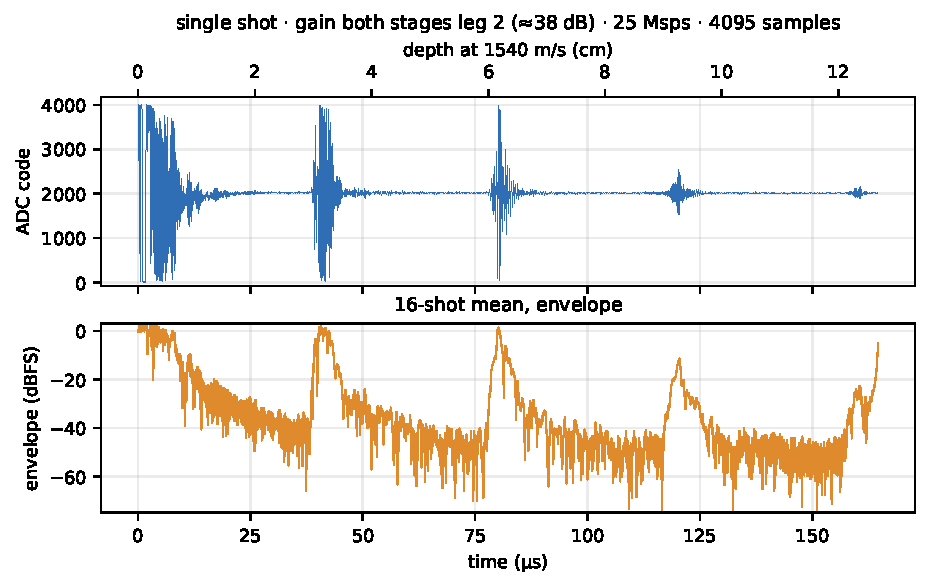
\includegraphics[width=\linewidth]{figures/aline.pdf}\\[-2pt]
{\footnotesize Single shot and 16-shot envelope, 3.3\,MHz piezo; echo train every \vechospacing\us{} (\vpathmm\,mm one way).}
\end{minipage}

\vspace{4pt}
\begin{figure}[H]
\centering
\begin{tikzpicture}[font=\scriptsize, >=Stealth, x=12.2mm, y=10mm,
  b/.style={draw, rounded corners=1.5pt, align=center, minimum height=9mm, minimum width=13mm, inner sep=2pt, fill=white},
  rp/.style={b, fill=accentlight},
  pic/.style={b, fill=orange!14},
  lab/.style={font=\tiny, fill=white, inner sep=1pt}]
  % row 1: control + transmit
  \node[b]   (usb) at (0,0)   {USB-C\\5\,V · CDC};
  \node[rp]  (rp)  at (2.6,0) {RP2354A\\150\,MHz · CLI\\link · ICSP};
  \node[rp]  (pio) at (5.2,0) {PIO pulser\\6.67\,ns steps};
  \node[b]   (drv) at (7.5,0) {TC4427\\driver};
  \node[b]   (fet) at (9.8,0) {Q1 P / Q2 N\\+5\,V / GND};
  \node[b]   (tx)  at (12.4,0) {\textbf{TX}\\SMA RF3\\U.FL RF1};
  \node[b]   (ldo) at (0,-1.7) {AP2112K\\3.3\,V LDO};
  % row 2: receive (right to left)
  \node[b]   (rx)  at (12.4,-3.6) {\textbf{RX}\\SMA RF22\\U.FL RF23};
  \node[b]   (lim) at (10.75,-3.6) {10\,nF +\\BAV99 ±0.6\,V};
  \node[b]   (lna) at (9.1,-3.6) {LNA BGA2817\\24\,dB};
  \node[pic] (oa1) at (7.45,-3.6) {OA1\\×1 … ×11};
  \node[pic] (oa2) at (5.8,-3.6) {OA2\\×1 … ×11};
  \node[b]   (flt) at (4.15,-3.6) {RC 2×\\100\,Ω/56\,pF};
  \node[pic] (adc) at (2.5,-3.6) {ADC2 + DMA\\12 bit, 25\,Msps};
  \node[b]   (mux) at (6.625,-2.05) {74HC4052 R\textsubscript{f} mux\\2.2/4.7/6.8/10\,k};
  % arrows
  \draw[->] (usb) -- (rp); \draw[->] (usb) -- node[lab,left]{5\,V} (ldo);
  \draw[->] (rp) -- (pio); \draw[->] (pio) -- node[lab,above]{GPIO8/9} (drv);
  \draw[->] (drv) -- (fet); \draw[->] (fet) -- (tx);
  \draw[->] (rx) -- (lim); \draw[->] (lim) -- (lna); \draw[->] (lna) -- (oa1); \draw[->] (oa1) -- (oa2);
  \draw[->] (oa2) -- (flt); \draw[->] (flt) -- (adc);
  \draw[<->] ($(rp.south)+(-0.25,0)$) -- node[lab,left,align=right]{UART 115\,200\\TRIG} ($(adc.north)+(-0.15,0)$);
  \draw[->, dashed, warn] ($(adc.north)+(0.45,0)$) |- ++(0,1.05) -| node[lab,pos=0.75,right,text=warn]{RDY\,↑ fires the pulse} ($(pio.south)+(-0.35,0)$);
  \draw[->] ($(pio.south)+(0.35,0)$) |- node[lab,pos=0.7,above]{GPIO25/23} (mux.west);
  \draw (mux.south -| oa2) -- (oa2.north); \draw (mux.south -| oa1) -- (oa1.north);
  % legend
  \node[rp,  minimum width=5mm, minimum height=3mm] (l1) at (0,-5.0) {}; \node[right=1mm of l1, font=\scriptsize] {RP2354A};
  \node[pic, minimum width=5mm, minimum height=3mm] (l2) at (2.0,-5.0) {}; \node[right=1mm of l2, font=\scriptsize] {PIC32AK1216GC41048 (200\,MHz)};
  \node[b,   minimum width=5mm, minimum height=3mm] (l3) at (6.4,-5.0) {}; \node[right=1mm of l3, font=\scriptsize] {discrete parts};
\end{tikzpicture}
\caption{Block diagram. The RP2354A owns USB, the command line, the pulser and the gain mux; the PIC32AK owns the two op-amp gain stages, the ADC and the DMA capture.}
\end{figure}

% ====================================================================== contents
\newpage
\tableofcontents
\vspace{6pt}
\begin{tcolorbox}[colback=accentlight,colframe=accent,arc=1mm,boxrule=0.5pt,title={\bfseries How to read this datasheet},fonttitle=\small]
\small Values marked \meas{} were measured on one board (RP2354A unique ID \vuid, firmware rp~\vrpfw{} / pic~\vpicfw{}, link protocol~\vproto; the released firmware rp~\rpfwrel{} / pic~\picfwrel{} has the same acquisition code, plus the LP5562 LED driver and new names)
with a 3.3\,MHz single-element piezo transducer connected (characterised in \hyperref[sec:piezo]{Annex~A}), at room temperature, powered from a PC USB port. Values marked \des{} come
from the schematic, the component datasheets or the firmware and were not independently measured. Every measurement can be
reproduced with the scripts in \texttt{docs/bench/2026-11-19-*/} of the repository (\repo); the raw captures are stored next to them.
There is a single unit: no min/max over production is available.
\end{tcolorbox}

% ====================================================================== 1 ratings
\section{Absolute maximum ratings and operating conditions}
\small
\begin{tabularx}{\linewidth}{@{}Xllp{62mm}@{}}
\toprule
\textbf{Parameter} & \textbf{Rating} & \textbf{Unit} & \textbf{Limited by}\\\midrule
USB VBUS (+5.0\,V rail) & 6.0 & V & AP2112K V\textsubscript{IN} max 6.5\,V; TC4427 VDD 18\,V; IRLML2244 V\textsubscript{DS} −20\,V \des\\
TX connector (net \cmd{Transducer}), externally applied & −0.3 … 5.3 & V & Q1/Q2 body diodes to +5\,V / GND \des\\
RX connector (net \cmd{TRANSDUCER}), DC & ±50 & V & C45 10\,nF series capacitor rating (0402, 50\,V) \des\\
RX connector, transient after C45 & clamped ±0.6 & V & D2 BAV99 to GND (215\,mA, 4\,A surge) \des\\
ADC node, test points H6, J1, J2 & −0.3 … AVDD+0.3 & V & PIC32AK pins; D1 BAT54S on the ADC node \des\\
Storage temperature & −40 … +85 & °C & components \des\\
\bottomrule
\end{tabularx}

\vspace{4pt}
\begin{tabularx}{\linewidth}{@{}Xrrrlp{50mm}@{}}
\toprule
\textbf{Recommended operating condition} & \textbf{Min} & \textbf{Typ} & \textbf{Max} & \textbf{Unit} & \textbf{Notes}\\\midrule
Supply (USB-C VBUS) & 4.75 & 5.0 & 5.25 & V & USB 2.0 port; also on CN1.33, H6.18 \des\\
Logic / analog rails & & 3.3 & & V & AP2112K (600\,mA) → DVDD, ferrite L2 → AVDD \des\\
AVDD (ADC full scale) & & 3.32 & & V & from the 0.8\,V band gap \meas\\
Ambient temperature & 0 & 25 & 70 & °C & all parts are industrial grade; characterised at 25\,°C only\\
Transducer & 1 & 3.3 & 7 & MHz & receive chain −6\,dB band set by the transducer; anti-alias 10.6\,MHz \des\\
\bottomrule
\end{tabularx}
\normalsize

% ====================================================================== 2 electrical characteristics
\section{Electrical characteristics}
Unless noted: USB 5\,V, 25\,°C, firmware defaults (\cmd{pe 200 500 25}, ADC trigger divider 4, single conversions, pattern correction on).
\begin{spec}{Transmit (pulser)}
Output levels & no load & & 0 / 5.0 & & V \des\\
Output states & & \multicolumn{3}{c}{+5\,V, GND clamp, Hi-Z} & \des\\
+5\,V phase $t_{hi}$ & programmable, default 200\,ns & 13.3 & 200 & 27\,300 & ns \des\\
Dead time (both FETs off) & programmable, default & 26.7 & 26.7 & 873 & ns \des\\
GND clamp phase $t_{lo}$ & programmable, default 500\,ns & 13.3 & 500 & 27\,300 & ns \des\\
Timing resolution & PIO clock = clk\_sys 150\,MHz & & 6.67 & & ns \des\\
Driver & TC4427 (MIC4427 alt.), 1.5\,A peak, 10\,Ω gate R & & & & \des\\
Switches & Q1 IRLML2244 (P), Q2 IRLML6244 (N) & & & & \des\\
Pulse to ADC start & main bang onset, all inputs & & \vonsetns & & ns \meas\\
Sample-comb phase vs pulse & \vEshots{} shots, main-bang fit, near-uniform over 1 sample & & \vEphispan{} / \vEphirms & & ns p-p / rms \meas\\
Whole-sample comb slips & echo at \vEsliptime\us{} / \vEsliptimeb\us{}, shots off by ±1 sample & & \vEslipa{} / \vEslipb & & \% \meas\\
Pulse-width optimum & max. echo amplitude, 3.3\,MHz probe & 75 & \vhibest & 130 & ns \meas\\
Effective pulse length & $t_{hi}$ + offset (fit, incl. dead time) & & +\vdeltaeff & & ns \meas\\
Dead zone (ring-down > 6\,σ) & any $t_{lo}$ 0–2\,µs, gain 0\,1\,0 & & \vdeadzone & & \textmu s \meas\\
\grp{Receive chain}
Input coupling & C45 + C3 = 5\,nF series, BAV99 ±0.6\,V clamp & & & & \des\\
Input termination & R17 after the LNA & & 51 & & Ω \des\\
LNA gain & BGA2817, specified at ≥ 250\,MHz & & 24 & & dB \des\\
Op-amp stage gain (each) & 1 + R\textsubscript{f}/1\,kΩ, R\textsubscript{f} 2.2/4.7/6.8/10\,k & 3.2 & & 11.0 & V/V \des\\
OA1 measured gain & legs 0…3 & 3.6 & & 10.2 & V/V \meas\\
OA2 measured gain & legs 0…3 & 3.7 & & 13.1 & V/V \meas\\
Unity setting (UGE) & per stage & & 1.00 & & V/V \des\\
Total programmable gain & 9 settings, \cmd{gain leg u1 u2} & 0 & & 42.5 & dB \meas\\
Anti-alias filter & 2-pole RC, 2 × (100\,Ω, 56\,pF) & & 10.6 & & MHz \des\\
Echo centre frequency & 3.3\,MHz probe, echo 1 & & \vfcen & & MHz \meas\\
Echo −6\,dB band & 3.3\,MHz probe & \vbwlo & & \vbwhi & MHz \meas\\
Echo −6\,dB envelope length & ⇒ axial resolution \vaxres\,mm & & \vpulselen & & ns \meas\\
\grp{ADC and acquisition}
Resolution & & & 12 & & bit \des\\
Full scale & = AVDD & & 3.32 & & V \meas\\
LSB & & & 0.81 & & mV \meas\\
Sample rate & divider 4 (default) & & \vfsdivfour & & Msps \meas\\
 & divider 10 / 20 / 40 & & \multicolumn{2}{l}{\vfsdivten{} / \vfsdivtwenty{} / \vfsdivforty} & Msps \meas\\
Sample-rate tolerance & PIC FRC 8\,MHz & −1.5 & & +1.5 & \% \des\\
Record length & & & 4095 & & samples \des\\
Record duration & default & & \vfilldivfour & & \textmu s \meas\\
ADC noise alone & internal band gap, SAMC 3 & & \vadcsigma & & LSB rms \meas\\
ADC noise-limited ENOB & full Nyquist band & & \vadcenob & & bit \meas\\
ENOB (datasheet, 1\,kHz sine) & DS70005592 AD34 & & 10.5 & & bit \des\\
Fixed pattern (period 4) & before correction / after & & 10.5 / 0.17 & & LSB rms \meas\\
\grp{System noise (ADC node, no pulse, transducer connected, correction on)}
Output noise, unity gain & full band / 1.5–5\,MHz & & \vnzunity{} / \vnzbandunity & & LSB rms \meas\\
Noise-limited ENOB, unity & full band / 1.5–5\,MHz & & \venobunity{} / \venobbandunity & & bit \meas\\
Output noise, 42.5\,dB & full band / 1.5–5\,MHz & & \vnzmax{} / \vnzbandmax & & LSB rms \meas\\
Input noise density, 42.5\,dB & at OA1 input, 1.5–5\,MHz & & \veninmax & & nV/$\sqrt{\text{Hz}}$ \meas\\
In-band dynamic range, 42.5\,dB & full-scale sine / noise & & \vdrmax & & dB \meas\\
\grp{Repeatability and throughput}
Echo amplitude repeatability & 16 shots, echo 3, gain 2\,0\,0 & & \vampcv & & \% CV \meas\\
Echo arrival jitter & 16 shots, cross-correlation & & \vjitter & & ns rms \meas\\
Averaging gain & 8 shots, aligned, host-side & & \vavggain & & dB \meas\\
Time per \cmd{pe} (end to end) & incl. 8190\,B at 115\,200\,Bd (\vxfer\,s) & & \vpetime & & s \meas\\
Captures needing a re-shot & ADC 40/60/60\,ns lock, build dependent & 0 & & \vretryrate & \% \meas\\
\grp{Link and control}
USB & full speed, CDC-ACM & & 12 & & Mbit/s \des\\
RP↔PIC link & UART 8N1 & & 115\,200 & & Bd \des\\
Ping round trip & \cmd{ping}, mean of \vpingn & & \vpingus & & \textmu s \meas\\
\end{spec}

% ====================================================================== 3 typical performance
\clearpage
\section{Typical performance characteristics}
\begin{figure}[H]
\centering
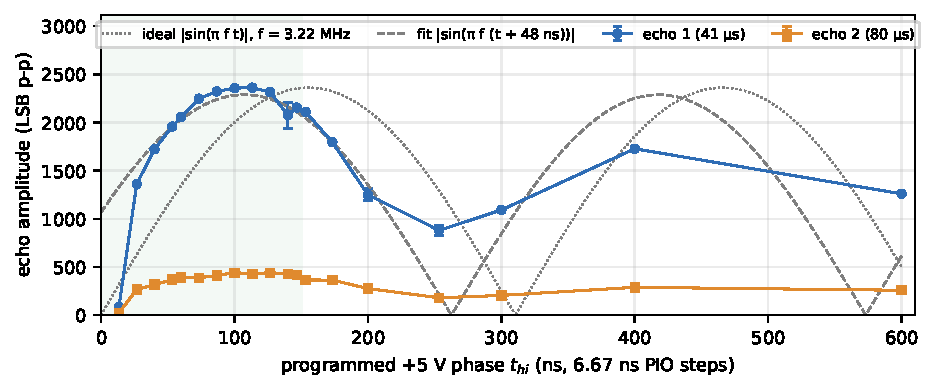
\includegraphics[width=0.94\textwidth]{figures/pulse_width.pdf}
\caption{Echo amplitude vs +5\,V phase length (gain 0\,1\,0, $t_{lo}$ = 500\,ns, mean of 2 shots, bars = half range)\meas.
\vhinpts{} points between 0 and 150\,ns (shaded). Dashed: spectrum of an ideal unipolar pulse at the echo centre frequency, $|\sin(\pi f_c t_{hi})|$.}
\end{figure}
\begin{figure}[H]
\centering
\begin{subfigure}[t]{0.43\textwidth}\centering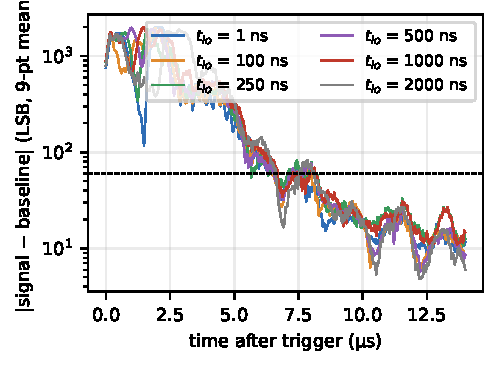
\includegraphics[width=\linewidth]{figures/clamp_ringdown.pdf}\caption{Ring-down after the pulse vs GND clamp length.}\end{subfigure}\hfill
\begin{subfigure}[t]{0.43\textwidth}\centering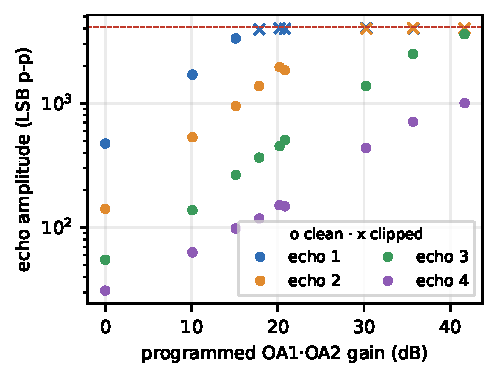
\includegraphics[width=\linewidth]{figures/gain_echoes.pdf}\caption{Echo amplitude vs programmed gain (4 echoes).}\end{subfigure}

\begin{subfigure}[t]{0.43\textwidth}\centering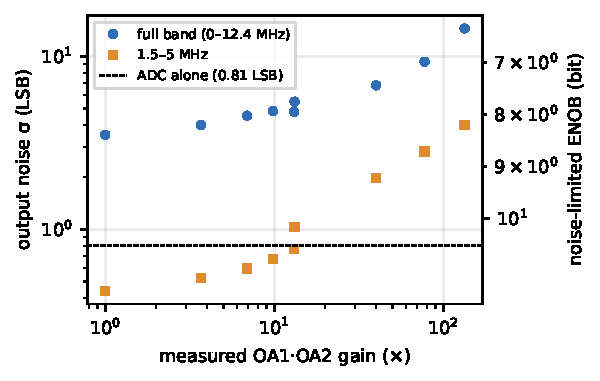
\includegraphics[width=\linewidth]{figures/noise_gain.pdf}\caption{Output noise and noise-limited ENOB vs gain.}\end{subfigure}\hfill
\begin{subfigure}[t]{0.43\textwidth}\centering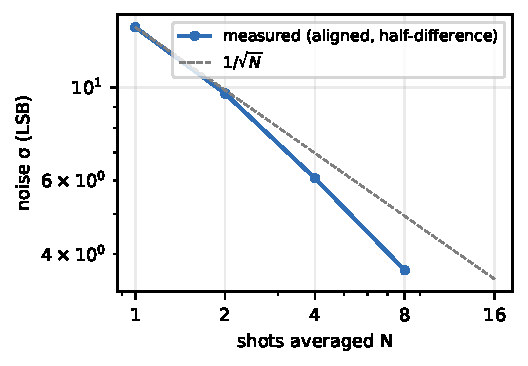
\includegraphics[width=\linewidth]{figures/averaging.pdf}\caption{Noise between the echoes vs number of aligned, averaged shots (gain 2\,0\,0).}\end{subfigure}
\caption{Pulser, gain and noise characteristics\meas. Echo amplitudes are peak-to-peak ADC codes at the ADC node (input 25), × = clipped.
Noise = standard deviation of a pulse-free record after the firmware pattern correction; noise-limited ENOB = $12-\log_2(\sigma\sqrt{12})$, distortion not included (upper bound).}
\end{figure}

\begin{figure}[H]
\centering
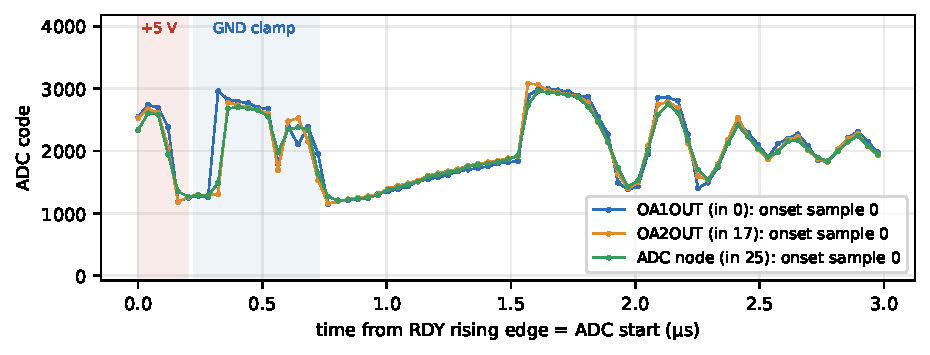
\includegraphics[width=\textwidth]{figures/main_bang.pdf}
\caption{Main bang at unity gain on three ADC inputs, aligned on the ADC start (RDY rising edge)\meas. The shaded areas are the programmed pulse phases.}
\end{figure}
\begin{figure}[H]
\centering
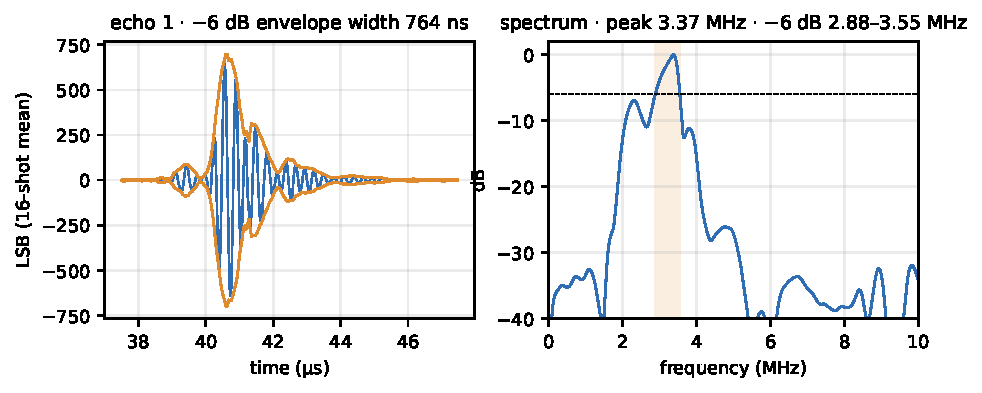
\includegraphics[width=\textwidth]{figures/echo_spectrum.pdf}
\caption{First echo (16-shot mean, gain 0\,1\,0): waveform with envelope and spectrum\meas.}
\end{figure}
\begin{figure}[H]
\centering
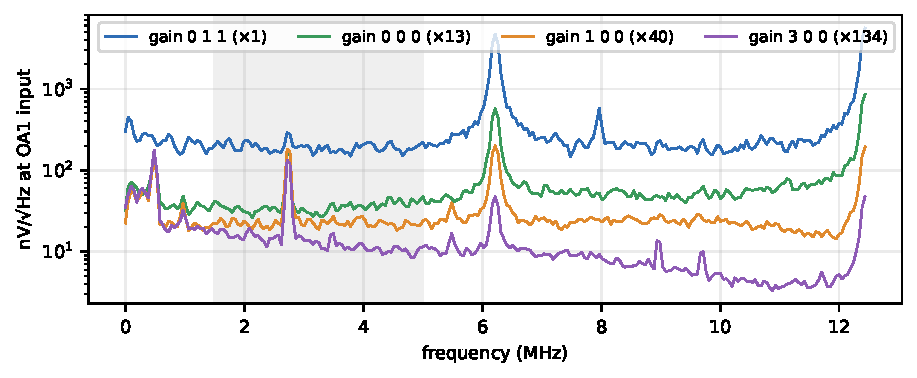
\includegraphics[width=\textwidth]{figures/noise_psd.pdf}
\caption{Noise density referred to the OA1 input (LNA output) at four gains\meas; shaded: 1.5–5\,MHz. Lines at 2.72\,MHz and 0.49\,MHz enter at the front end; fs/4 and fs/2 residues remain at 6.21 and 12.43\,MHz.}
\end{figure}

% ====================================================================== 4 functional description
\section{Functional description}
\subsection{Power}
USB-C VBUS is the +5.0\,V rail (CC pins with 5.1\,kΩ pull-downs: sink only). It feeds the pulser driver and FETs directly and the
AP2112K-3.3 LDO, which makes +3V3\_DVDD; a 120\,Ω ferrite bead (L2) derives +3V3\_AVDD for the LNA, the op-amp bias dividers, the
gain mux and the PIC analog supply. The RP2354A's internal switching regulator makes its 1.1\,V core (L1 3.3\,µH).
Supply current was not measured (no meter in the loop); the LNA alone takes 20\,mA\des.

\subsection{Clocks}
\begin{itemize}
  \item RP2354A: 12\,MHz oscillator U7 → clk\_sys 150\,MHz (pico-sdk 2.1.0 default). The pulser PIO runs at clk\_sys: 6.67\,ns steps.
  \item PIC32AK: internal 8\,MHz FRC (±1.5\,\%) → PLL1 VCO 1000\,MHz → 200\,MHz CPU (CLKGEN1), 250\,MHz ADC clock (CLKGEN6, T\textsubscript{AD} 16\,ns), 200\,MHz SCCP time base (CLKGEN12, 5\,ns).
  \item OSC1 32.768\,kHz feeds the LP5562 LED driver only (the firmware selects the LP5562 internal clock instead).
\end{itemize}

\subsection{Pulser}
Two RP GPIOs drive the dual non-inverting driver U3, which drives a complementary totem on the \cmd{Transducer} net:
\begin{center}\small
\begin{tabular}{@{}llll@{}}\toprule
\textbf{GPIO8 (“PWM\_H”)} & \textbf{GPIO9 (“PWM\_L”)} & \textbf{FETs} & \textbf{TX output}\\\midrule
0 & 1 & both off & released (Hi-Z), idle\\
0 & 0 & Q1 (P) on & +5\,V\\
1 & 1 & Q2 (N) on & GND clamp\\
1 & 0 & both on & \textcolor{warn}{shoot-through — never generated}\\\bottomrule
\end{tabular}\end{center}
The sequence is produced by a PIO state machine (\texttt{firmware/rp2354/pulser.pio}) from one 32-bit word per shot, so it is
cycle-exact and independent of the CPU. Phase lengths: +5\,V = $t_{hi}$, both off = dead time (≥ 4 cycles = 26.7\,ns), GND = $t_{lo}$,
then released. In pulse-echo mode the state machine waits for RDY low then high; the PIC raises RDY one instruction before
starting the ADC trigger timer, so the pulse and sample 0 coincide to within a few tens of ns (\vonsetns\,ns measured).

\begin{figure}[H]
\centering
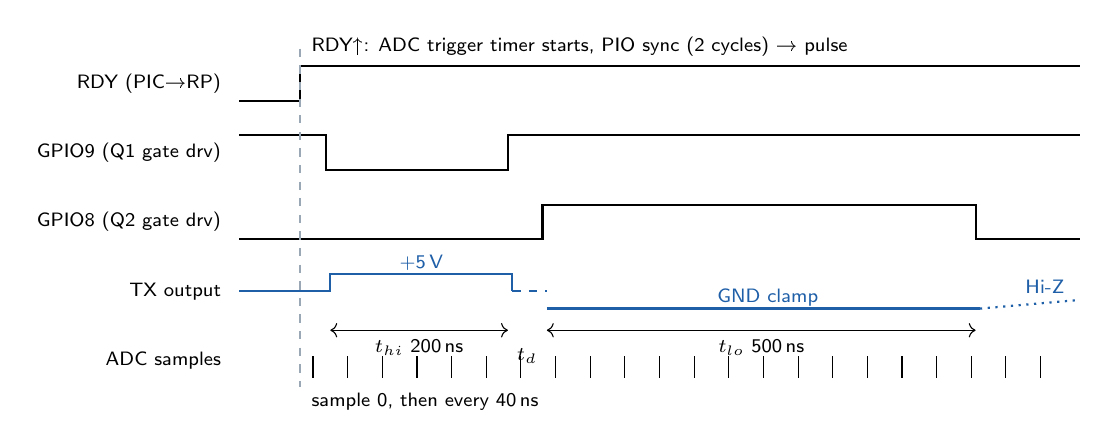
\begin{tikzpicture}[font=\scriptsize, x=11mm, y=5.5mm]
  \foreach \y/\n in {0/RDY (PIC→RP), -1.6/GPIO9 (Q1 gate drv), -3.2/GPIO8 (Q2 gate drv), -4.8/TX output, -6.4/ADC samples} \node[anchor=east] at (-0.2,\y+0.4) {\n};
  \draw[thick] (-0.1,0) -- (0.6,0) -- (0.6,0.8) -- (9.6,0.8);
  \draw[thick] (-0.1,-0.8) -- (0.9,-0.8) -- (0.9,-1.6) -- (3.0,-1.6) -- (3.0,-0.8) -- (9.6,-0.8);
  \draw[thick] (-0.1,-3.2) -- (3.4,-3.2) -- (3.4,-2.4) -- (8.4,-2.4) -- (8.4,-3.2) -- (9.6,-3.2);
  \draw[thick, accent] (-0.1,-4.4) -- (0.95,-4.4) -- (0.95,-4.0) -- (3.05,-4.0) -- (3.05,-4.4);
  \draw[thick, accent, dashed] (3.05,-4.4) -- (3.45,-4.4);
  \draw[thick, accent] (3.45,-4.8) -- (8.45,-4.8); \draw[thick, accent, dotted] (8.45,-4.8) -- (9.6,-4.6);
  \node[accent] at (2.0,-3.75) {+5\,V};
  \node[accent] at (6.0,-4.55) {GND clamp};
  \node[accent] at (9.2,-4.3) {Hi-Z};
  \foreach \x in {0.75,1.15,...,9.4} \draw (\x,-6.4) -- (\x,-5.9);
  \draw[decorate,decoration={brace,amplitude=3pt}] (0.95,-1.85) -- node[below=2pt]{} (0.95,-1.85);
  \draw[<->] (0.95,-5.3) -- node[below]{$t_{hi}$ 200\,ns} (3.0,-5.3);
  \draw[<->] (3.45,-5.3) -- node[below]{$t_{lo}$ 500\,ns} (8.4,-5.3);
  \node at (3.22,-5.9) {$t_d$};
  \draw[dashed, rule] (0.6,1.2) -- (0.6,-6.6);
  \node[anchor=west] at (0.62,1.25) {RDY↑: ADC trigger timer starts, PIO sync (2 cycles) → pulse};
  \node[anchor=west] at (0.62,-6.95) {sample 0, then every 40\,ns};
\end{tikzpicture}
\caption{Pulse-echo timing (not to scale). Driver propagation (TC4427 ≈ 20\,ns) and the PIO input synchroniser add a fixed delay.}
\end{figure}

\subsection{Receive chain}
\begin{enumerate}
  \item \textbf{Protection and coupling}: C45 10\,nF in series (blocks DC on a shared TX/RX cable), D2 BAV99 anti-parallel to GND (±0.6\,V), C3 10\,nF into the LNA.
  \item \textbf{LNA}: BGA2817 wideband MMIC, 24\,dB at RF; C32 10\,nF, D3 BAV99 clamp, 51\,Ω termination R17 to GND, R29 0\,Ω.
  \item \textbf{OA1}: PIC op amp 1, non-inverting, IN+ biased at AVDD/2 by R33/R34 through R37 (C40 330\,pF coupling), R\textsubscript{g} = R28 1\,kΩ + C43 100\,nF to GND (unity DC gain), R\textsubscript{f} via 74HC4052 section 1.
  \item \textbf{OA2}: identical (C1 330\,pF, R31/R32/R38 bias, R30 + C44, 74HC4052 section 2).
  \item \textbf{Anti-alias}: R67/C86 + R68/C87 (100\,Ω/56\,pF each), D1 BAT54S clamp to GND/AVDD, into AD2AN9 (pin 4).
\end{enumerate}

\begin{table}[H]\centering\small
\caption{Gain settings (\cmd{gain <leg> <u1> <u2>}). Programmed = 1 + R\textsubscript{f}/R\textsubscript{g}; measured from echo ratios\meas.}
\begin{tabular}{@{}lcccccc@{}}\toprule
\textbf{Command} & \textbf{R\textsubscript{f}} & \textbf{OA1} & \textbf{OA2} & \textbf{Programmed} & \textbf{Measured} & \textbf{Noise}\\
& & & & \textbf{dB} & \textbf{dB} & \\\midrule
\cmd{gain 0 1 1} & — & ×1 & ×1 & 0.0 & 0.0 & Table~\ref{tab:noise}\\
\cmd{gain 0 1 0} & 2.2\,k & ×1 & ×3.2 & 10.1 & 11.3 & \\
\cmd{gain 1 1 0} & 4.7\,k & ×1 & ×5.7 & 15.1 & 16.8 & \\
\cmd{gain 2 1 0} & 6.8\,k & ×1 & ×7.8 & 17.8 & 19.8 & \\
\cmd{gain 3 1 0} & 10\,k & ×1 & ×11 & 20.8 & 22.3 & \\
\cmd{gain 0 0 0} & 2.2\,k & ×3.2 & ×3.2 & 20.2 & 22.4 & \\
\cmd{gain 1 0 0} & 4.7\,k & ×5.7 & ×5.7 & 30.2 & 32.0 & \\
\cmd{gain 2 0 0} & 6.8\,k & ×7.8 & ×7.8 & 35.7 & 37.8 & \\
\cmd{gain 3 0 0} & 10\,k & ×11 & ×11 & 41.7 & 42.5 & \\\bottomrule
\end{tabular}\end{table}
Both 4052 sections share the select lines, so OA1 and OA2 always use the same R\textsubscript{f} leg; a stage is bypassed (×1) with the
op-amp's internal unity-gain switch (AMPxCON1.UGE). The LNA gain (24\,dB, not measured at 3\,MHz) comes on top.

\subsection{Acquisition}
SCCP1 produces a 20\,ns trigger comb (CLKGEN12 / 4); the 32\,ns ADC2 conversion takes every second trigger, giving a uniform
40\,ns sample period (24.86\,Msps measured against the PIC's own timer). DMA0 moves each 16-bit result to RAM (40\,ns per transfer at
200\,MHz is the DMA ceiling). At some start phases the ADC locks to a 40/60/60\,ns pattern (fill 226\us{} instead of 164.7\us);
since pic~0.1.25 the PIC flags it (status \cmd{slow}, no payload) and \cmd{pe}/\cmd{acq} re-fire within milliseconds. Since rev~0.3
the cause is better understood: it is a \emph{per-PLL-lock} state (after a lock, either almost no capture or 85–100\,\% of them come
out slow), and the PIC now re-locks at boot until its test captures are uniform (\S\ref{sec:lock}).
The phase of the sample comb relative to the pulse varies from shot to shot over one full sample period: see
\S\ref{sec:combphase}. Align shots (cross-correlation on a strong echo, sub-sample shift) before averaging.
After the capture the PIC removes the period-4 fixed pattern (below) and replies with a header line; the RP then pulls the
8190 bytes over SPI (\S\ref{sec:link}) and prints them on the USB console (decimal, or base64 with \cmd{fmt b64}).

\subsection{Sample-comb phase and slips (E3)}\label{sec:combphase}
A campaign of \vEshots{} \cmd{pe} shots (\texttt{docs/bench/2026-11-19-jitter/}, rp~1.1.1/pic~1.1.0, gain 2\,0\,0)
measured the pulse time $\varphi$ against the sample comb in each shot. The main bang is purely electrical, so it was used for this:
the \vEshots{} shots sample it at different phases, which gives a 1\,ns equivalent-time template, and each shot's $\varphi$ is a
least-squares fit to it (a fit one sample away is $\sim10^4\times$ worse, so there is no wrap ambiguity).
\begin{itemize}
  \item $\varphi$ spans \vEphispan\,ns (one 40.2\,ns sample), \vEphirms\,ns rms (uniform: 11.6\,ns). It is close to uniform, but not
        exactly (KS distance \vEksd, $p$ = \vEksp): the histogram has some clustering (periodogram peak \vEclusterr{} at
        \vEclusterp\,ns, near the 4\,ns period of the 250\,MHz ADC clock).
  \item Shots are independent: lag-1 autocorrelation \vEacone. A random 0–50\,ms pause before each shot changes nothing.
  \item \textbf{Whole-sample slips.} Compared with $\varphi$, the strong echo at \vEsliptime\us{} is off by exactly ±1 sample in
        \vEslipa\,\% of shots, and the echo at \vEsliptimeb\us{} in \vEslipb\,\%. So during a capture the comb sometimes gains or
        loses a whole 40\,ns period, more often the longer the capture runs. This is not visible in the fill time, whose resolution is 80\,ns. The slipped
        shots cluster at particular start phases ($\varphi\approx-10$ and $+12$\,ns), which points at a marginal
        trigger/conversion lock at those phases: the same mechanism as the 40/60/60\,ns slow lock (E2), in a milder form.
        Aligned shots agree with $\varphi$ to \vEresid\,ns rms.
\end{itemize}
Consequence for averaging: align each shot on the echo of interest, not on the main bang, and reject shots whose late echoes
disagree by a whole sample. Firmware fix (not done): start the SCCP1 trigger from the ADC clock domain, or time-stamp every
conversion.
\begin{figure}[h]\centering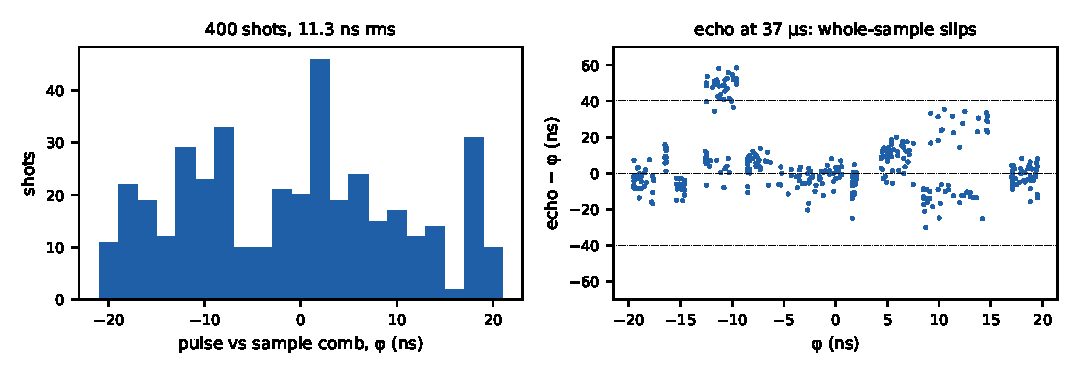
\includegraphics[width=0.9\textwidth]{figures/comb_phase.pdf}
\caption{Left: pulse vs sample-comb phase over \vEshots{} shots. Right: echo delay minus $\varphi$ (slow acoustic drift removed);
bands at ±40.2\,ns are whole-sample slips.}\end{figure}

\subsection{Fixed-pattern correction (period-4 pattern)}\label{sec:pc}
\textbf{The pattern.} Every external ADC input carries a pattern locked to the sample clock with a period of four samples: one
phase in four sits $\approx$\,\xPcLow\,LSB below the other three, \xPcRaw\,LSB rms over the four phase means (median of \xPcN{}
captures, gain ×10, no pulse\meas). It does not scale with the analog gain and the internal band-gap input is free of it, so it is
injected at the ADC (digital/DMA activity at fs/4 coupling into the sample-and-hold or the references), not in the front end. In the
spectrum it is the line pair at fs/4 = 6.2\,MHz and fs/2 = 12.4\,MHz. Its phase (which of the four samples is low) is random from
capture to capture, so it cannot be calibrated once: it is estimated in every capture.

\textbf{The correction, step by step} (PIC firmware, \texttt{acq.c} \texttt{acq\_pc\_apply}, after every single-conversion capture):
\begin{enumerate}[nosep]
  \item Skip the first 64 samples (main bang and settling).
  \item Over samples 64…4094, compute the mean of each phase $k = i \bmod 4$ and the overall mean.
  \item Offset of phase $k$ = its mean minus the overall mean, kept in 1/16\,LSB (\cmd{pc} prints the four values).
  \item Subtract the offset of its phase from every sample (0…4094), round, clamp to 0…4095.
\end{enumerate}
Echoes and noise average out over the $\approx$\,1000 samples of each phase because they are not locked to fs/4.
Measured\meas: residual pattern \xPcCor\,LSB rms after correction (median of \xPcN{} captures; \xPcBad\,\% of captures above 2\,LSB).
The estimator assumes one phase for the whole capture: a whole-sample comb slip (E3) in the middle of a capture swaps the phases for
the rest of it and leaves part of the pattern in that capture. A block-wise robust variant was tried against a tgc switch transient
and gave the same residual (\texttt{docs/bench/2026-11-22-pc-robust/}), so the simple estimator is kept. \cmd{pc 0} disables the
correction (it is also skipped for \cmd{navg} > 1, \cmd{samc} > 0 and oversampling).
\begin{figure}[H]\centering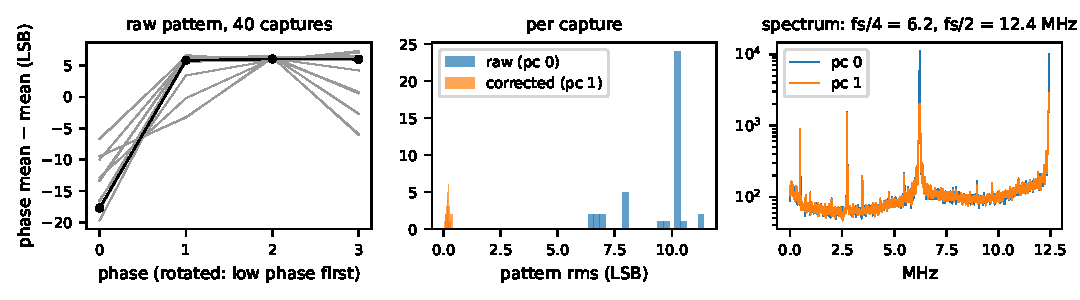
\includegraphics[width=\textwidth]{figures/ext_pc.pdf}
\caption{Period-4 pattern\meas. Left: phase means minus the mean, \xPcN{} raw captures, rotated so the low phase comes first.
Middle: pattern rms per capture, raw (\cmd{pc 0}) and corrected (\cmd{pc 1}). Right: mean spectra; the fs/4 and fs/2 lines go away.}\end{figure}

\textbf{The signal before and after, computed on the host.} To see exactly what the correction does to the samples, \xPcN{} captures
were taken with the correction \emph{off} (\cmd{pc 0}) and the PIC's algorithm was applied to them on the host, bit for bit
(integer arithmetic, 1/16\,LSB, same rounding; \texttt{analyze.py} \texttt{pc\_host}, results in \texttt{pc\_host.npz}):
\begin{itemize}[nosep]
  \item \textbf{Raw}: in a clean capture one phase sits \xPcOffB\,LSB from the mean and the three others at \xPcOffA, \xPcOffC,
        \xPcOffD\,LSB — the four per-phase histograms are separated (Fig.~\ref{fig:pcsignal}, top right); in the time trace every
        fourth sample dips.
  \item \textbf{Corrected}: the four offsets are subtracted and the four histograms coincide (middle left); the dips are gone and
        the trace is the noise of the chain. The sample standard deviation falls from \xPcHostRaw{} to \xPcHostCor\,LSB (mean of
        \xPcN{} captures); the PIC's own corrected captures (other shots) give \xPcPicCor\,LSB — the same.
  \item \textbf{Slipped captures}: in \xPcSlipN{} of \xPcN{} captures (\xPcSlip\,\%) the low phase moves by one sample in the middle of the
        record (E3 comb slip, bottom left). One set of four offsets cannot fit both halves, so two populations remain after the
        correction (bottom right) and the fs/4 line is only partly removed in those captures. A per-segment estimate would fix it at
        the cost of noisier offsets; not done yet.
\end{itemize}
\begin{figure}[H]\centering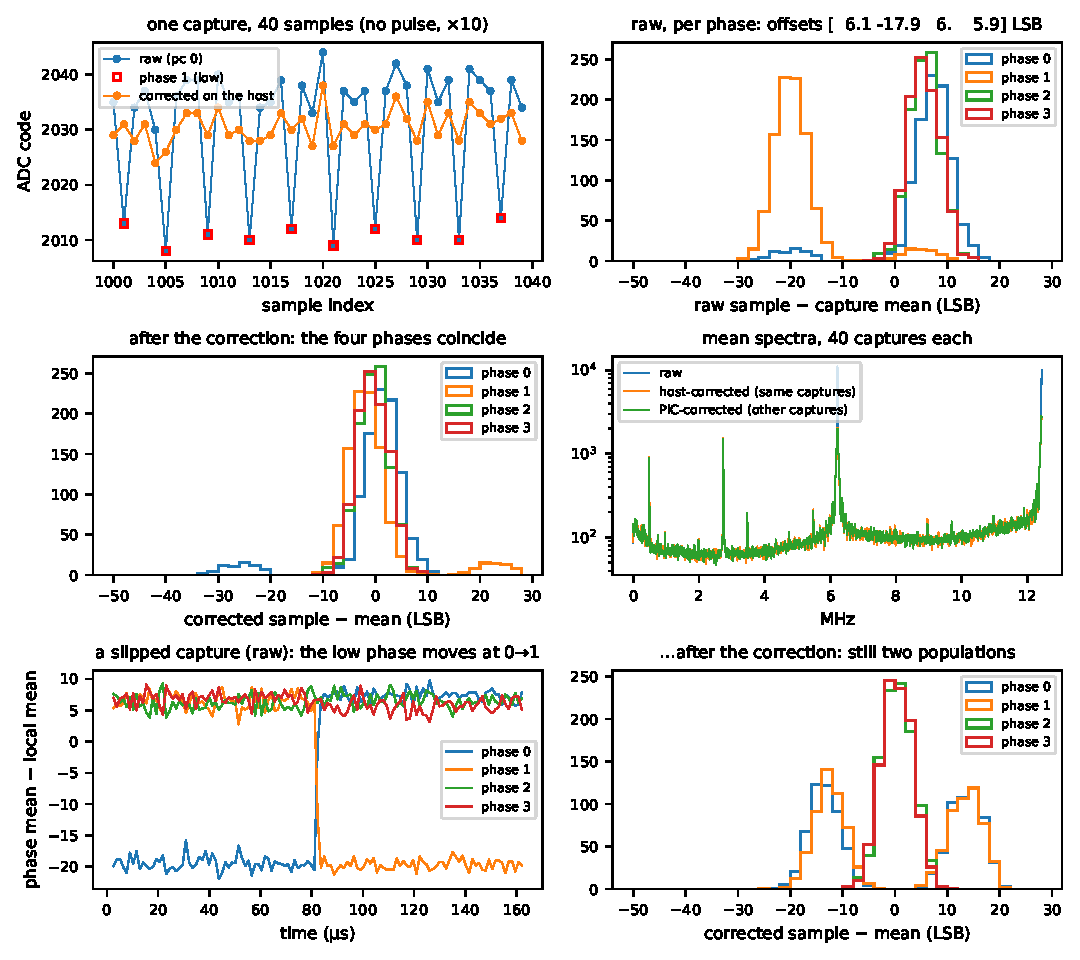
\includegraphics[width=\textwidth]{figures/ext_pc_signal.pdf}
\caption{The period-4 correction applied on the host to raw captures (no pulse, gain ×10)\meas. Top: 40 samples of a clean
capture, raw and corrected (red squares: the low phase), and its per-phase histograms (raw). Middle: the same after the
correction; mean spectra (raw, host-corrected, PIC-corrected). Bottom: a slipped capture — the phase means along the record, and
the two populations left after the correction.}\label{fig:pcsignal}\end{figure}

\subsection{Noise summary}
\begin{table}[H]\centering\small
\caption{Output noise at the ADC node vs gain (firmware correction on, no pulse)\meas. Band = 1.5–5\,MHz with the 2.72\,MHz line notched;
e\textsubscript{n} referred to the OA1 input (= LNA output) using the measured gain.}\label{tab:noise}
\begin{tabular}{@{}lrrrrrrr@{}}\toprule
\textbf{Setting} & \textbf{Prog.} & \textbf{Meas.} & \multicolumn{2}{c}{\textbf{Full band}} & \multicolumn{2}{c}{\textbf{1.5–5\,MHz}} & \textbf{e\textsubscript{n} @ OA1 in}\\
& \textbf{dB} & \textbf{dB} & \textbf{LSB} & \textbf{ENOB} & \textbf{LSB} & \textbf{ENOB} & \textbf{nV/$\sqrt{\text{Hz}}$}\\\midrule
\noiserows
\bottomrule\end{tabular}\end{table}
Below $\approx$\,20\,dB the ADC itself sets the in-band floor; above $\approx$\,32\,dB the front end dominates. At full gain the
in-band noise referred to the LNA input is $\approx$\,0.85\,nV/$\sqrt{\text{Hz}}$ if the LNA gives 24\,dB — the thermal noise of
50\,Ω (0.91\,nV/$\sqrt{\text{Hz}}$) — so extra analog gain mostly amplifies front-end noise; averaging is the better lever.

% ====================================================================== 4b on-PIC processing (rev 0.3)
\section{Capture link and on-PIC processing}
All measurements in this section: campaign of \xCampDate{} on board~3 with the Annex~A transducer (echoes at \xEchoAt\us{} =
\xEchoAmm\,mm and \xEchoBt\us), firmware \xCampFw; data as compressed NumPy files and scripts in
\texttt{docs/bench/2026-11-22-datasheet-ext/} (\texttt{campaign.py} records, \texttt{analyze.py} makes the figures and numbers).

\subsection{RP↔PIC data link}\label{sec:link}
The capture payload (4095 × u16) no longer travels over the 115\,200\,Bd UART (0.71\,s): the RP pulls it as one SPI frame.
\begin{enumerate}[nosep]
  \item The PIC answers a capture command with its header line only and keeps the samples.
  \item The RP sends \cmd{SPIX}. The PIC drops RDY, preloads its SPI1 transmit FIFO, raises RDY (= ``clock now'').
  \item The RP (SPI0 master, mode 1, CS on GPIO5) clocks 12 + 2n bytes: \cmd{A5 5A 'M' '1'}, n, sequence number, the samples
        (little-endian u16) and a CRC-32 over all of it; the PIC computes the CRC while feeding the FIFO and drops RDY at the end.
  \item The RP checks magic, n (against the header) and the CRC; on any error it asks again over the UART (\cmd{UTX}) and counts it.
\end{enumerate}
\begin{table}[H]\centering\small
\caption{\cmd{linktest}: the PIC fills its buffer with a 16-bit LFSR, the RP pulls it 200 times and checks every word\meas.}
\begin{tabular}{@{}rrrrrrl@{}}\toprule
\textbf{SPI (MHz)} & \textbf{ok} & \textbf{errors} & \textbf{per frame (ms)} & \textbf{SPIX→RDY (µs)} & \textbf{clocking (ms)} & \textbf{= UART copy}\\\midrule
\xLinkRows
\bottomrule\end{tabular}\end{table}
12.5\,MHz is the default (\cmd{link spi 25} is also clean); the 455\us{} SPIX→RDY is the 5-character request on the UART. The text
sent to the host was the next limit: \cmd{fmt b64} sends the samples as base64 (\xFmtBsixKB\,KB instead of \xFmtTextKB\,KB), and a
complete \cmd{acq} from Python takes \textbf{\xFmtBsix\,ms} instead of \xFmtText\,ms\meas. The Python library selects it on connect.

\subsection{Envelope detection}\label{sec:env}
Two envelope detectors are available: one on the PIC (\cmd{env}, only the envelope crosses the link) and one on the host
(library and live viewer, from the full RF A-line). Both are shown on the same first echo in Fig.~\ref{fig:envsteps}.

\textbf{On the PIC (\cmd{env <dec> [shots [in]]}, firmware \texttt{pe\_ext.c} \texttt{pe\_env}), step by step:}
\begin{enumerate}[nosep]
  \item \textbf{Capture.} The RP arms the pulser; the PIC captures 4095 samples at 25\,Msps with the standard settings (div 4, samc 0,
        navg 1, whatever the last \cmd{acq} used) and applies the period-4 correction (\S\ref{sec:pc}).
  \item \textbf{Baseline.} The mean of the 4095 samples is the baseline (the echoes are sparse, so the mean is the bias point).
  \item \textbf{Rectify.} Each sample becomes $|x - \text{mean}|$.
  \item \textbf{Integrate and dump.} The rectified samples are summed over blocks of \cmd{dec} = 4…64 samples and divided by \cmd{dec}:
        one value per block, kept in 1/16\,LSB. This is a boxcar low-pass plus decimation: 4095/dec values, dec × 40.2\,ns apart.
        For a sine of amplitude $A$ it gives $2A/\pi$ (the mean of $|\sin|$).
  \item \textbf{Average over shots.} With \cmd{shots} > 1 the RP fires again and the PIC adds each new envelope into a running
        32-bit sum (the second capture buffer); the current average is written back for transfer. Envelopes can be averaged
        although the sample comb moves by up to one sample from shot to shot (E3): 40\,ns is small against a 1\us{} envelope.
  \item \textbf{Transfer.} The RP pulls the 4095/dec values over SPI and prints them (1/16\,LSB).
\end{enumerate}
\textbf{On the host (library \texttt{minus.live.hilbert\_envelope}, live viewer):} (1) take the RF A-line; (2) remove its mean;
(3) FFT, zero the negative frequencies and double the positive ones (analytic signal); (4) inverse FFT and take the magnitude.
This gives the instantaneous amplitude $A$ at every sample (no decimation, no $2/\pi$ factor) but needs the whole A-line on the host.

Checks\meas: an emulation of steps 2–4 on 16 host-side \cmd{pe} shots matches the PIC's 16-shot \cmd{env 8} with correlation
\xEnvCorr{} (energy ratio \xEnvRatio\,\%), and $2/\pi$ × the Hilbert envelope lies on both. One \cmd{env 8} takes \xEnvTimeA\,ms end
to end, \cmd{env 8 16} \xEnvTimeB\,ms.
\begin{figure}[H]\centering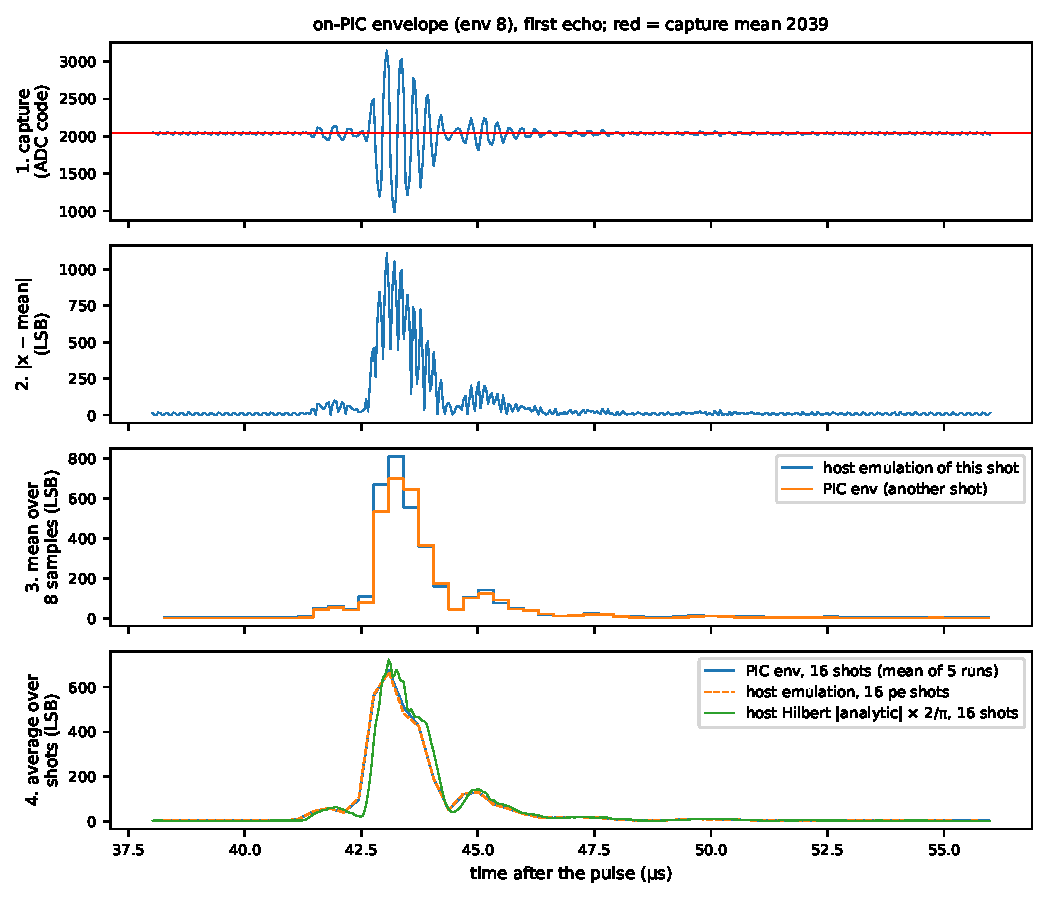
\includegraphics[width=\textwidth]{figures/ext_env_steps.pdf}
\caption{Envelope detection on the first echo, gain ×\xRefGain\meas. 1: the capture and its mean; 2: rectified; 3: integrate-and-dump
over 8 samples (host emulation of this shot and the PIC's \cmd{env 8} of another shot); 4: averages over 16 shots — PIC, host
emulation and the host Hilbert envelope × $2/\pi$.}\label{fig:envsteps}\end{figure}
\begin{table}[H]\centering\small
\caption{\cmd{env} on the echoes (gain ×\xRefGain, 5 runs per setting)\meas. Floor = mean / run-to-run spread in the echo-free
55–78\us{} window (LSB); the spread falls roughly as $1/\sqrt{\text{shots}}$.}
\begin{tabular}{@{}rrrcccr@{}}\toprule
\textbf{dec} & \textbf{ns/value} & \textbf{values} & \textbf{floor, 1 shot} & \textbf{4 shots} & \textbf{16 shots} & \textbf{echo peak (LSB)}\\\midrule
\xEnvRows
\bottomrule\end{tabular}\end{table}
\begin{figure}[H]\centering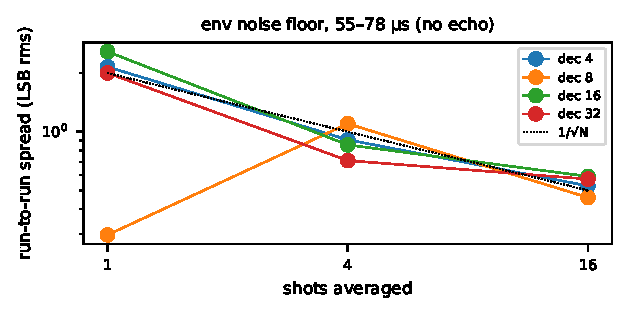
\includegraphics[width=0.55\textwidth]{figures/ext_env_shots.pdf}
\caption{Run-to-run spread of the \cmd{env} noise floor vs shots averaged\meas.}\end{figure}

\subsubsection*{Band-pass envelope on the PIC (\cmd{envbp})}\label{sec:envbp}
Between the echoes, most of what \cmd{env} reports is not noise in the probe band: it is the fs/4 and fs/2 residues of the
period-4 pattern (6.2 / 12.4\,MHz) and the 2.74\,MHz interference line (E5). Filtering to the probe band before detecting removes
it. The textbook way is an FFT, keep the band, inverse FFT, take the magnitude; a 4096-point complex FFT does not fit in the PIC's
16\,KB of RAM, so \cmd{envbp} does the equivalent convolution, evaluated only where an output value is needed.

\textbf{\cmd{envbp <dec> [shots [in [fc\_kHz [bw\_kHz]]]]}, step by step} (firmware \texttt{pe\_ext.c} \texttt{pe\_envbp}; defaults
fc 3300\,kHz, bw 2500\,kHz):
\begin{enumerate}[nosep]
  \item \textbf{Capture} as for \cmd{env} (pulse, standard settings, period-4 correction).
  \item \textbf{Filter design}, from the measured sample period $\Delta t$: a Gaussian window $g_k = e^{-k^2\Delta t^2/2\sigma_t^2}$ with
        $\sigma_t = 1/(2\pi\sigma_f)$ and $\sigma_f = \text{bw}/2.355$ (bw = full width at half maximum of the pass band), cut at
        $\pm3\sigma_t$ (21 taps for 2.5\,MHz), times $e^{j2\pi f_c k\Delta t}$. In frequency this is a Gaussian pass band centred on
        $+f_c$ only: band-pass and Hilbert transform in one complex filter.
  \item \textbf{Baseline}: subtract the capture mean.
  \item \textbf{Filter at the output points only}: for block $j$ (centre sample $c = j\cdot\text{dec} + \text{dec}/2$),
        $I + jQ = \sum_k h_k\,x_{c+k}$ — the analytic, band-limited signal at that sample.
  \item \textbf{Magnitude}: $2\sqrt{I^2+Q^2}/\sum_k g_k$ = the amplitude of the in-band signal (a sine of amplitude $A$ at $f_c$
        gives $A$), in 1/16\,LSB.
  \item \textbf{Average over shots and transfer} exactly as \cmd{env} (running 32-bit sum, 4095/dec values over SPI).
\end{enumerate}
The pass band must be \emph{tapered}: on the recorded echoes a brick-wall 2–6\,MHz FFT mask rings (sinc in time) and spreads the
first echo into the floor (43.2\,dB peak/floor), a raised-cosine 2–6\,MHz band gives 53.0\,dB and the Gaussian 3.3/2.5\,MHz
62.2\,dB, against 49.8\,dB for both \cmd{env} and a full-band Hilbert envelope (host prototype on 16 shots,
\texttt{bandpass\_env.py}, Fig.~\ref{fig:bpenv}). On the PIC\meas: \cmd{envbp} gains \xBpGain\,dB of peak/floor over \cmd{env} on a
single shot, in \xBpTime\,ms per shot (Table~\ref{tab:envbp}). A narrower band lowers the floor further but lengthens the
envelope (less axial resolution): 2.5\,MHz is a compromise for this 3.3\,MHz probe.
\begin{figure}[H]\centering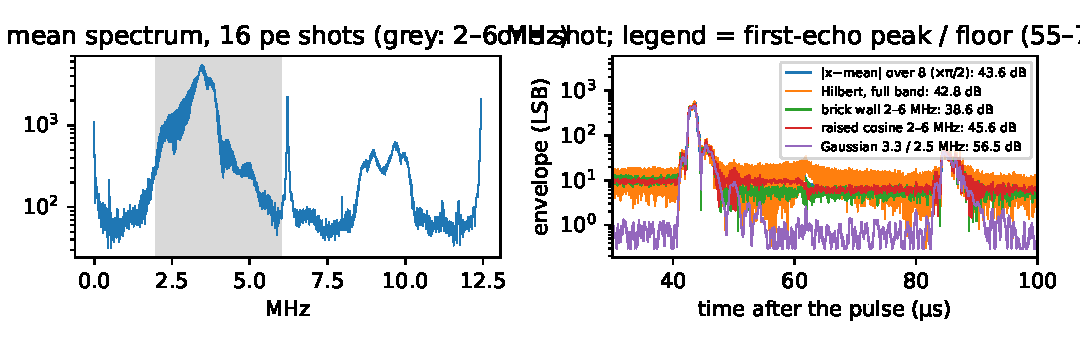
\includegraphics[width=\textwidth]{figures/ext_bpenv.pdf}
\caption{Host prototype of the band-pass envelope on 16 recorded shots: spectrum with the 2–6\,MHz band (left); one shot with
each envelope, legend = first-echo peak / floor 55–78\us{} (right)\meas.}\label{fig:bpenv}\end{figure}
\begin{table}[H]\centering\small
\caption{On the PIC, first echo, gain ×\xRefGain, dec 8, 5 runs per setting\meas. Floor = rms of the envelope in 55–78\us{} (LSB).}\label{tab:envbp}
\begin{tabular}{@{}lrrrrr@{}}\toprule
\textbf{Detector (fc / bw kHz)} & \textbf{peak (LSB)} & \textbf{floor, 1 shot} & \textbf{peak/floor (dB)} & \textbf{floor, 16 shots} & \textbf{dB, 16 shots}\\\midrule
\xBpRows
\bottomrule\end{tabular}\end{table}
\begin{figure}[H]\centering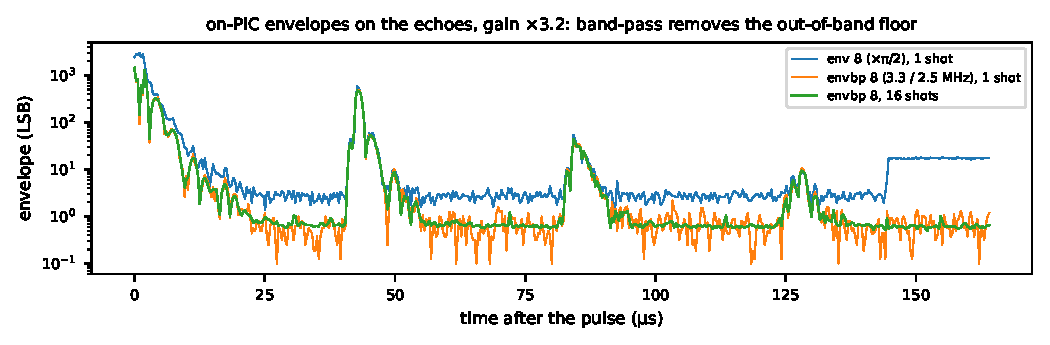
\includegraphics[width=\textwidth]{figures/ext_envbp.pdf}
\caption{\cmd{env} vs \cmd{envbp} on the PIC, same session\meas.}\end{figure}

\subsection{Time of flight}\label{sec:tof}
\textbf{\cmd{tof <thr> [blank\_ns [in [ref]]]}, step by step} (firmware \texttt{pe\_tof}):
\begin{enumerate}[nosep]
  \item The ADC channel's digital comparator is armed out of [ref − thr, ref + thr] (ref = 2048 when not given); its flag tells
        whether any sample of the capture left that window (reported, not used for the result).
  \item Pulse + capture with the standard settings, period-4 correction.
  \item If ref was not given, the baseline is the capture mean.
  \item The PIC scans from the sample \cmd{blank\_ns}/40 onward for the first $|x - \text{ref}| > \text{thr}$, then for the largest
        $|x - \text{ref}|$ in the next 64 samples.
  \item One line goes back: index, time, one-way depth at 1540\,m/s, peak, ref, comparator flag — no A-line transfer
        (\xTofTime\,ms per shot end to end).
\end{enumerate}
\begin{table}[H]\centering\small
\caption{\cmd{tof} on the first echo, 25\us{} blank, gain ×\xRefGain, 50 shots per threshold\meas. ``Host'' = the same search
run on 30 host-side \cmd{pe} captures.}
\begin{tabular}{@{}rrrrrrrr@{}}\toprule
\textbf{thr} & \textbf{found \%} & \textbf{mean (µs)} & \textbf{std (ns)} & \textbf{peak} & \textbf{host mean} & \textbf{host std} & \textbf{flag \%}\\\midrule
\xTofRows
\bottomrule\end{tabular}\end{table}
The result is the first RF half-cycle that crosses the threshold, not the envelope onset: with a threshold close to the peak of one
cycle, noise and the shot-to-shot comb phase pick that cycle or the next (one 3.3\,MHz period = 303\,ns), which is the large spread
at thr 100. Choose thr well between two cycle peaks, or use \cmd{env} for an envelope-based timing.
\begin{figure}[H]\centering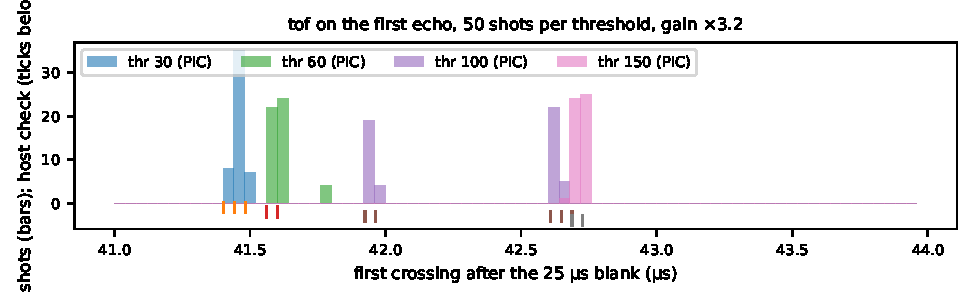
\includegraphics[width=0.85\textwidth]{figures/ext_tof.pdf}
\caption{\cmd{tof} crossing times per threshold\meas.}\end{figure}

\subsection{Live view}
\texttt{python3 -m minus.live} (desktop window) and \texttt{minus.live.LiveView(dev)} (Jupyter, ipywidgets) show each shot as the
A-line, its envelope in dB and an M-mode image (the last 120 envelopes, depth down, time to the right). Modes: \cmd{pe}, \cmd{acq},
\cmd{env}, \cmd{envbp}, \cmd{tof} (the \cmd{tof} result as a marker). On the bench transducer\meas: \xLiveFpsPe{} frames/s in \cmd{pe}
mode and \xLiveFpsBp{} in \cmd{envbp} mode (the window is drawn with Agg here; Jupyter is slower, $\approx$\,5 frames/s, because each
frame is sent as an image).
\begin{figure}[H]\centering
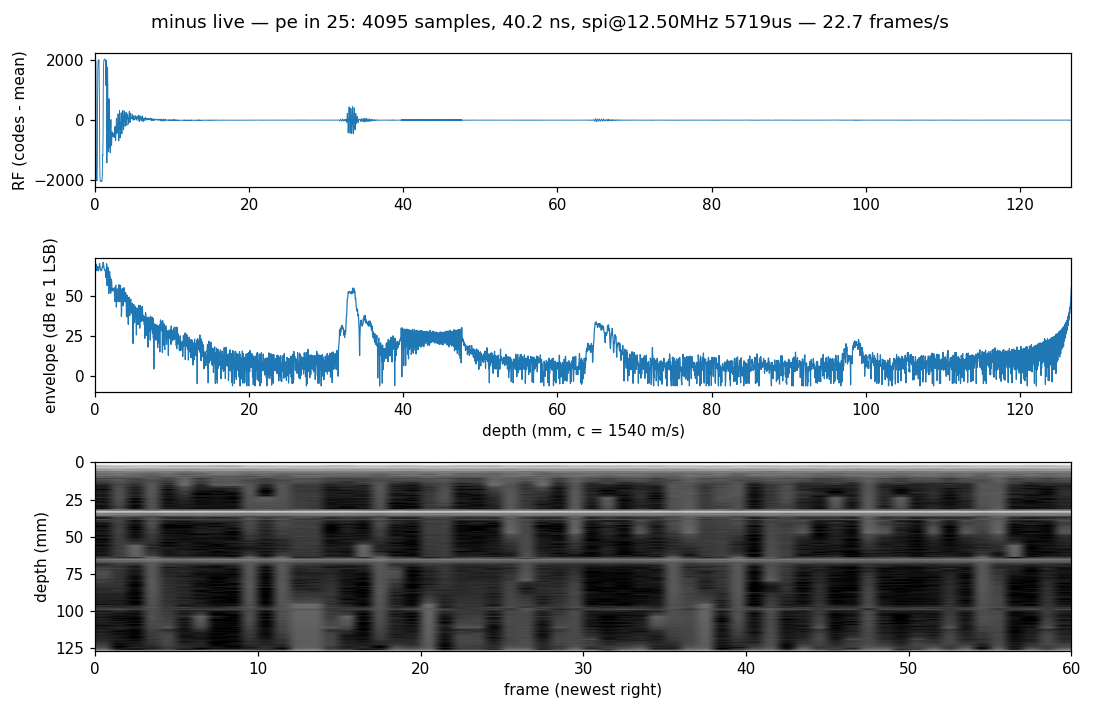
\includegraphics[width=0.49\textwidth]{figures/ext_live_pe.png}\hfill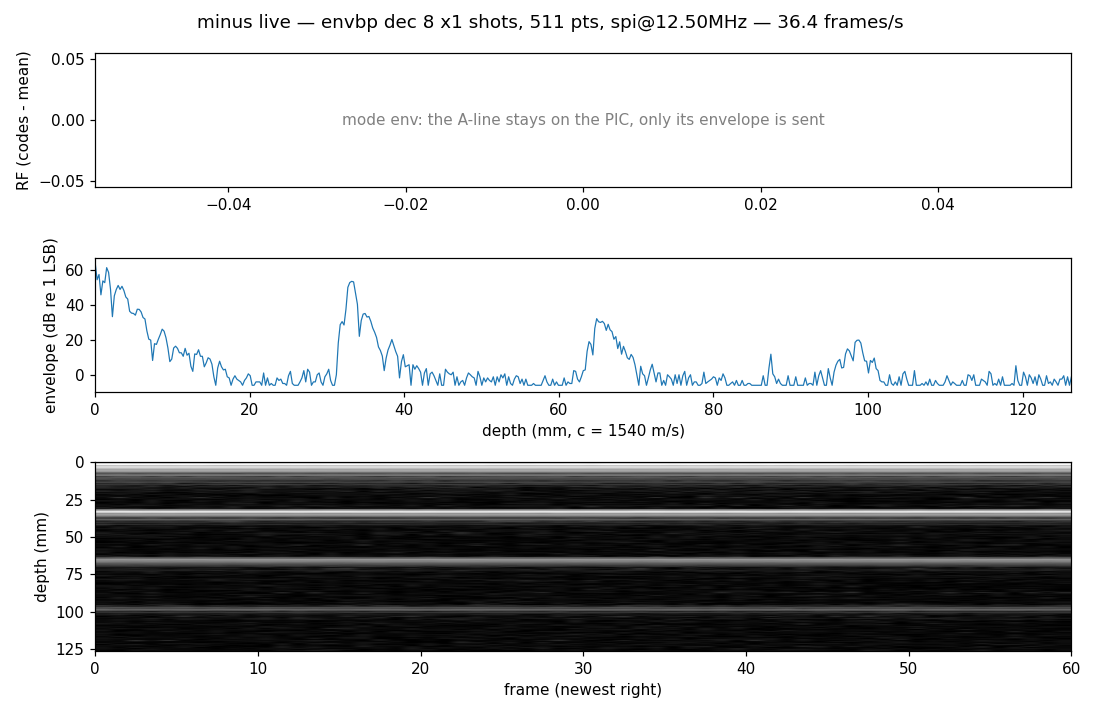
\includegraphics[width=0.49\textwidth]{figures/ext_live_envbp.png}
\caption{The live viewer on the bench echoes, gain ×3.2\meas. Left: \cmd{pe} mode (RF, Hilbert envelope, M-mode). Right: \cmd{envbp}
mode (the PIC sends only the band-pass envelope; the RF panel stays empty).}\end{figure}

\subsection{Oversampling (\cmd{acqos})}
\cmd{acqos 4|16 [in [pe]]} sets the ADC channel to hardware oversampling (MODE 11): every trigger runs 4 or 16 back-to-back 32\,ns
conversions and returns one 13- or 14-bit result (2× or 4× a 12-bit code). The trigger period is raised to fit: \xOsDtB{} and
\xOsDtC\,ns per sample\meas, i.e. a 0.76 / 2.32\,ms window. On a DC level the noise falls from \xOsNoiseA{} to \xOsNoiseB{} and
\xOsNoiseC\,LSB rms\meas. One pulse, averaging inside each sample. \textbf{It is not an RF mode:} at 5.4 / 1.77\,Msps a 3.3\,MHz echo
aliases (Nyquist 2.7 / 0.88\,MHz) and the 128 / 512\,ns average cancels it — the first echo keeps \xOsEchoRatioB\,\% / \xOsEchoRatioC\,\%
of its \cmd{pe} amplitude. Use it for slow signals and long, low-noise windows; use \cmd{pe}, \cmd{env} or \cmd{tof} for echoes.
\begin{figure}[H]\centering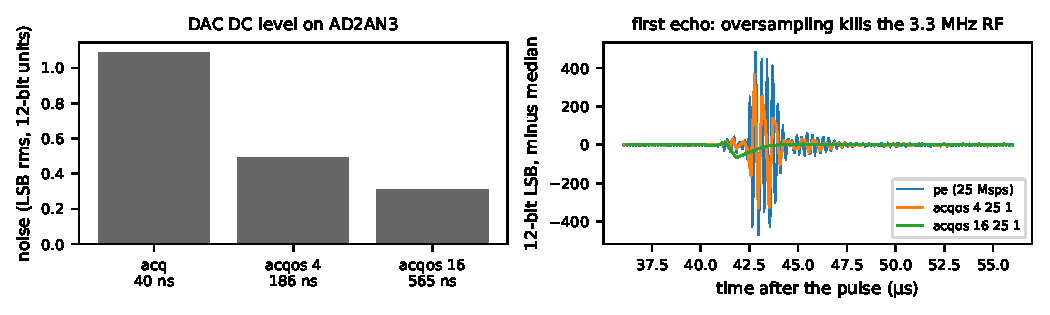
\includegraphics[width=\textwidth]{figures/ext_acqos.pdf}
\caption{\cmd{acqos}: noise on a DAC DC level (left) and the first echo with \cmd{pe} vs oversampling (right)\meas.}\end{figure}

\subsection{Time-gain steps (\cmd{tgc})}
\cmd{tgc <t\_us> <leg> [<t\_us> <leg> …]} switches the 74HC4052 gain leg of both stages at up to four times after the pulse, during
every capture; the leg set by \cmd{gain} is restored after. Measured with a step from ×10 to ×61 at \xTgcAt\us, between the first
echo and the later ones\meas: the first echo (before the step) is unchanged (×\xTgcBefore), the third echo (after the transient)
grows ×\xTgcRatio{} (a constant ×61 gives ×\xTgcConst), and the second echo at \xEchoBt\us{} falls inside the switch transient
(\xTgcAt–\xTgcEnd\us): it still comes out ×\xTgcInB{} (×\xTgcInBc{} for a constant ×61), but on top of the settling tail. Each switch costs $\approx$\,2\us{} of saturation and $\approx$\,15\us{} of
settling: the 4052 breaks before it makes, so the op-amp feedback opens for a moment. Place steps at least 17\us{} before the
echoes of interest; the Python \texttt{Capture.tgc\_valid()} masks 17\us{} after each step.
\begin{figure}[H]\centering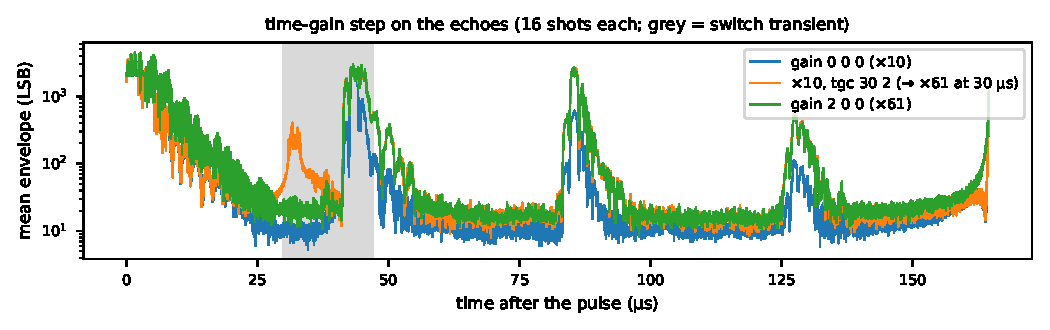
\includegraphics[width=\textwidth]{figures/ext_tgc.pdf}
\caption{Time-gain step on the echoes (mean envelope of 16 shots)\meas.}\end{figure}

\subsection{DAC test signal}
\cmd{dac off|dc <code>|tri <lo> <hi> <slope>|sine <hz> [amp [mid]]} drives DACOUT1 (U9 pin 3, H6.16), which is also ADC2 input
AD2AN3: \cmd{acq 4 0 19} reads it with no wiring. Codes 205…3890 = 5…95\,\% of 3.3\,V; the PDM DAC settles in 0.75–2\us.
\cmd{tri} runs in hardware (half period (hi−lo)·16/slope × 4\,ns) and is the reference to use during captures; \cmd{sine} is fed by
DMA and makes 20–25\,Msps captures \cmd{slow} (bus contention) — the PIC pauses it during its lock check.
Measured\meas: the DC sweep is linear to within \xDacInl\,LSB (ADC code = \xDacGain\,× DAC code + \xDacOff); the triangle has a period of
\xTriPer\us{} (nominal 24.58) and the same values over SPI and UART; a 20\,kHz, 50-point sine captured at 10\,Msps (\cmd{acq 20 0 19},
where the capture DMA has the slack to share the bus) fits at \xSineF\,kHz with \xSineRes\,LSB rms residual = \xSineSinad\,dB SINAD
— the DAC (pulse density, 1\us{} steps) limits it, so it is a shape reference, not an ADC test source. At 25\,Msps
\xSineSlow{} of \xSineN{} captures came back \cmd{slow} with the sine running, and the PIC's lock check was unaffected.
\begin{figure}[H]\centering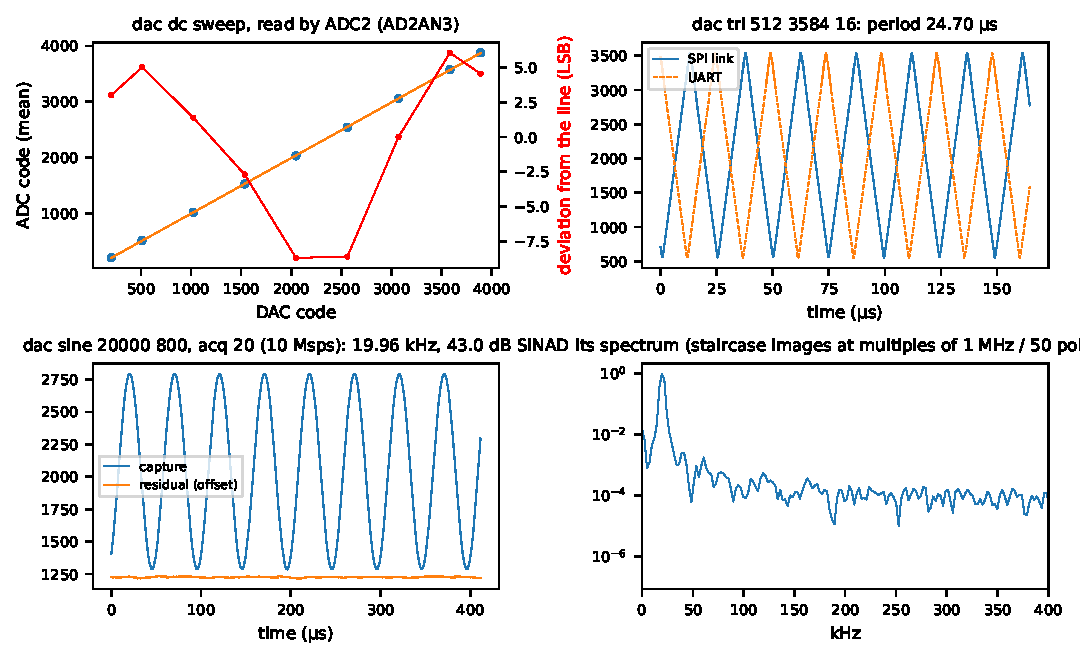
\includegraphics[width=\textwidth]{figures/ext_dac.pdf}
\caption{DAC test signal read back by ADC2 on AD2AN3\meas: DC sweep with the deviation from a line, triangle over SPI and UART,
sine with fit residual, and its spectrum.}\end{figure}

\subsection{PLL lock check at boot (E2)}\label{sec:lock}
The 40/60/60\,ns ``slow'' lock is set when PLL1 locks: the phase between its CPU/SCCP divider (VCO/5) and its ADC divider (VCO/4)
decides it, and a new lock re-rolls it (12 boots before the fix: 6 clean, 6 with 85–100\,\% slow captures). At boot the PIC runs
8 test captures and re-locks PLL1 (up to 12 times) until none is slow; \cmd{raw LOCK?} reports \cmd{LOCK <locks> <slow of 8>}, and
the RP sends \cmd{RELOCK} if 3 captures in a row come back slow. Over \xLockBoots{} boots\meas: all \xLockOk{} uniform (20 of 20
captures each), \xLockFirst{} on the first lock, at most \xLockMax{} locks (mean \xLockMean).

% ====================================================================== 5 pinout
\section{Connectors and pin assignment}
\begin{figure}[H]\centering
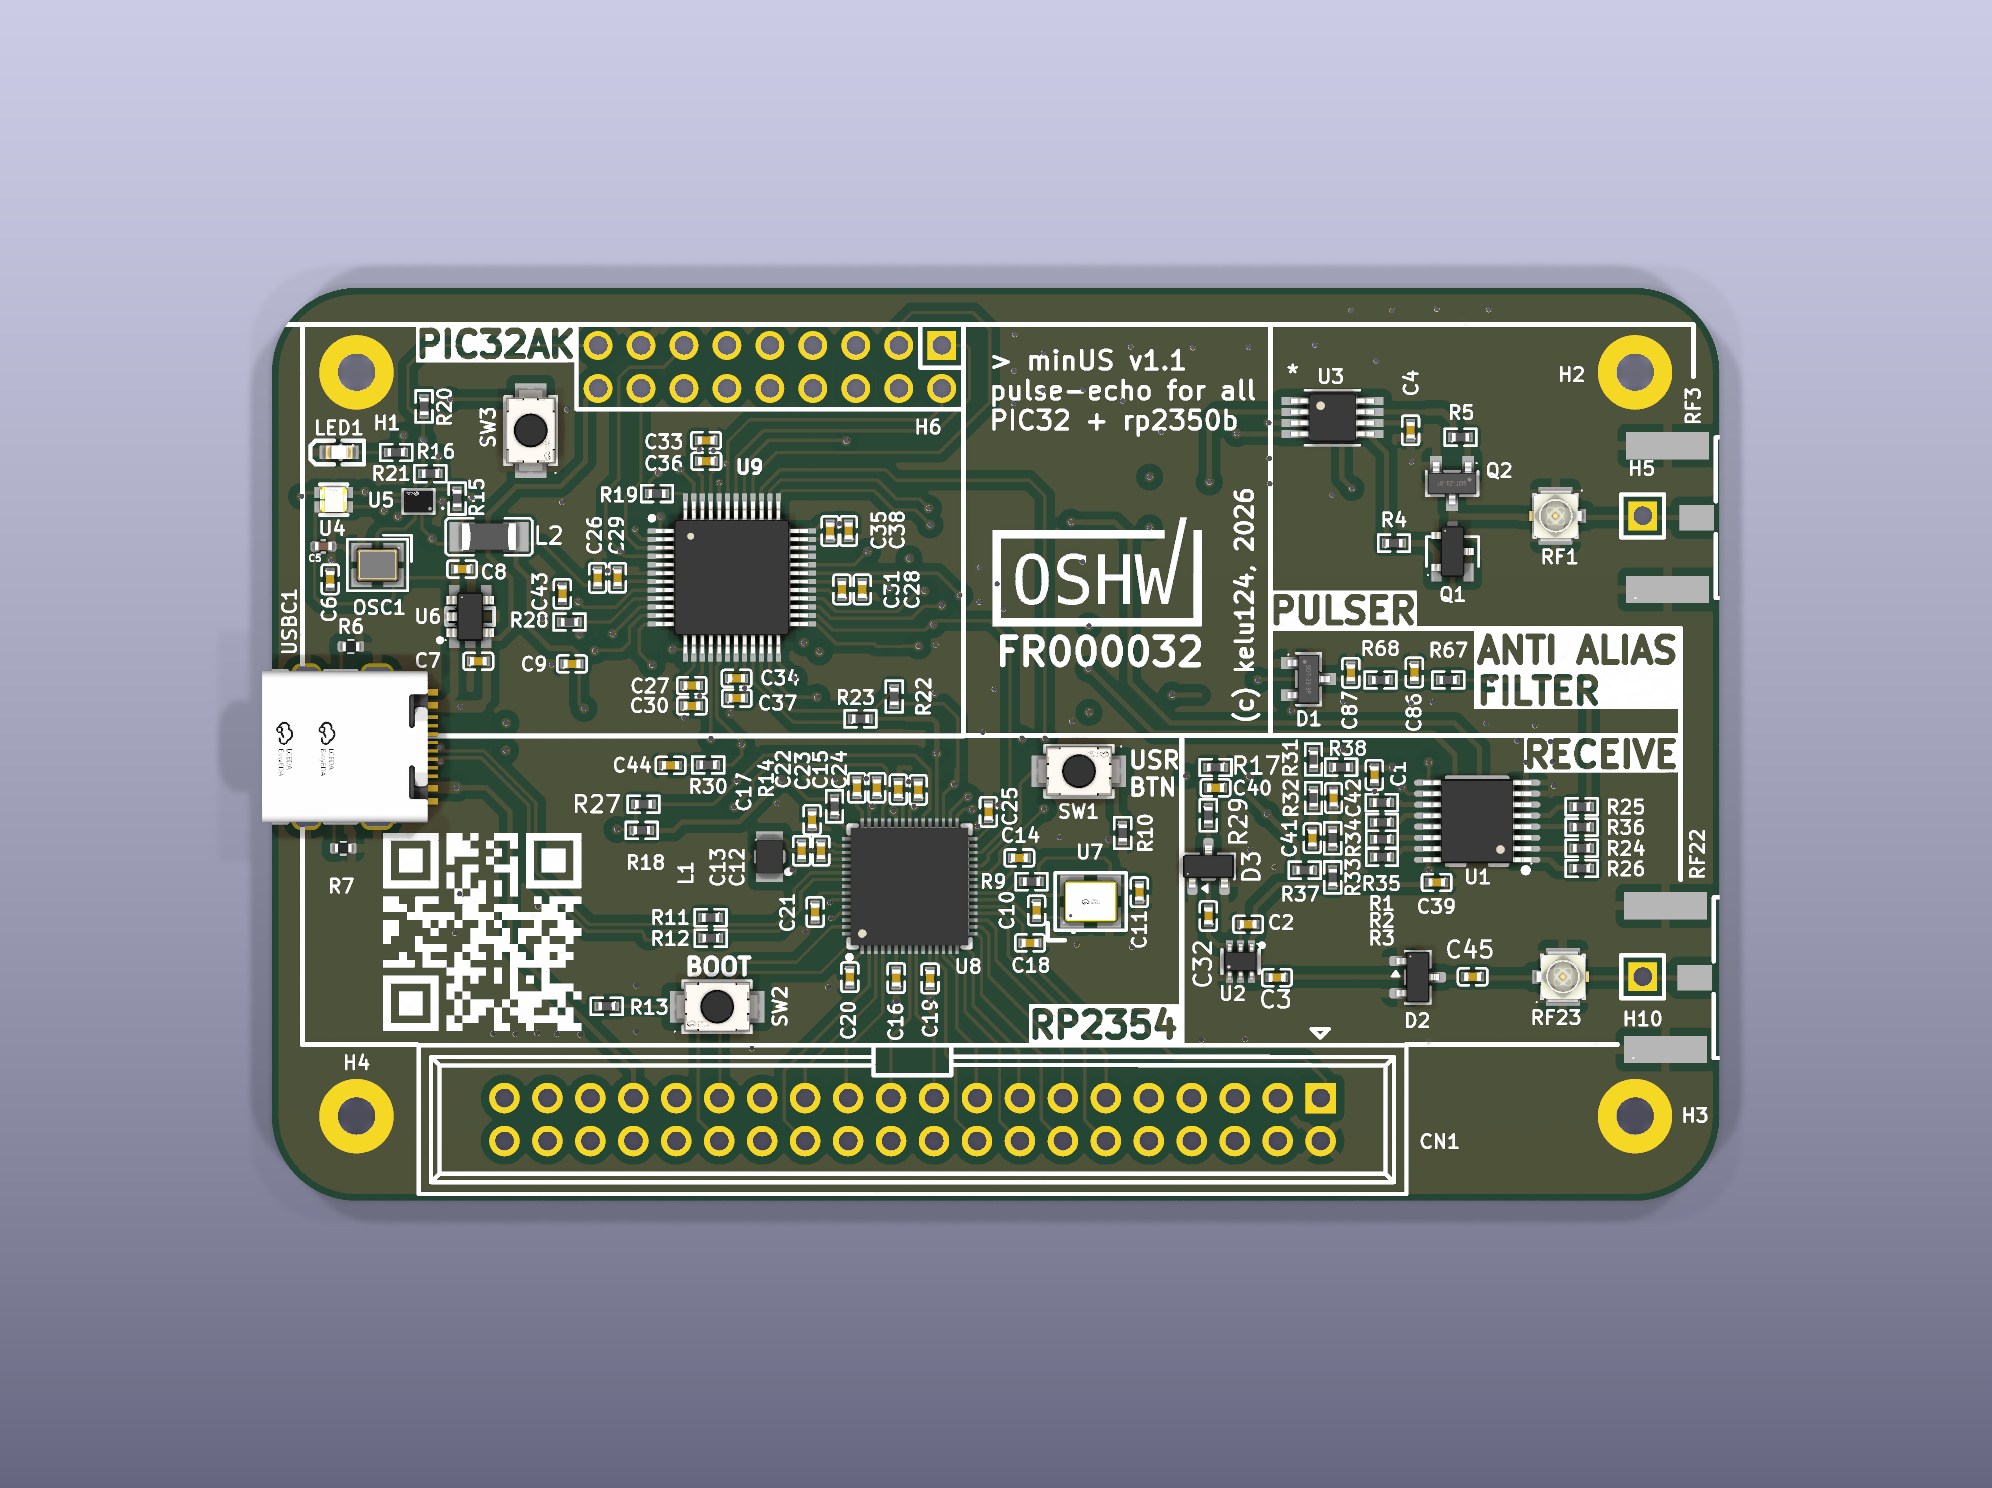
\includegraphics[width=0.48\textwidth]{figures/minUS_F.png}\hfill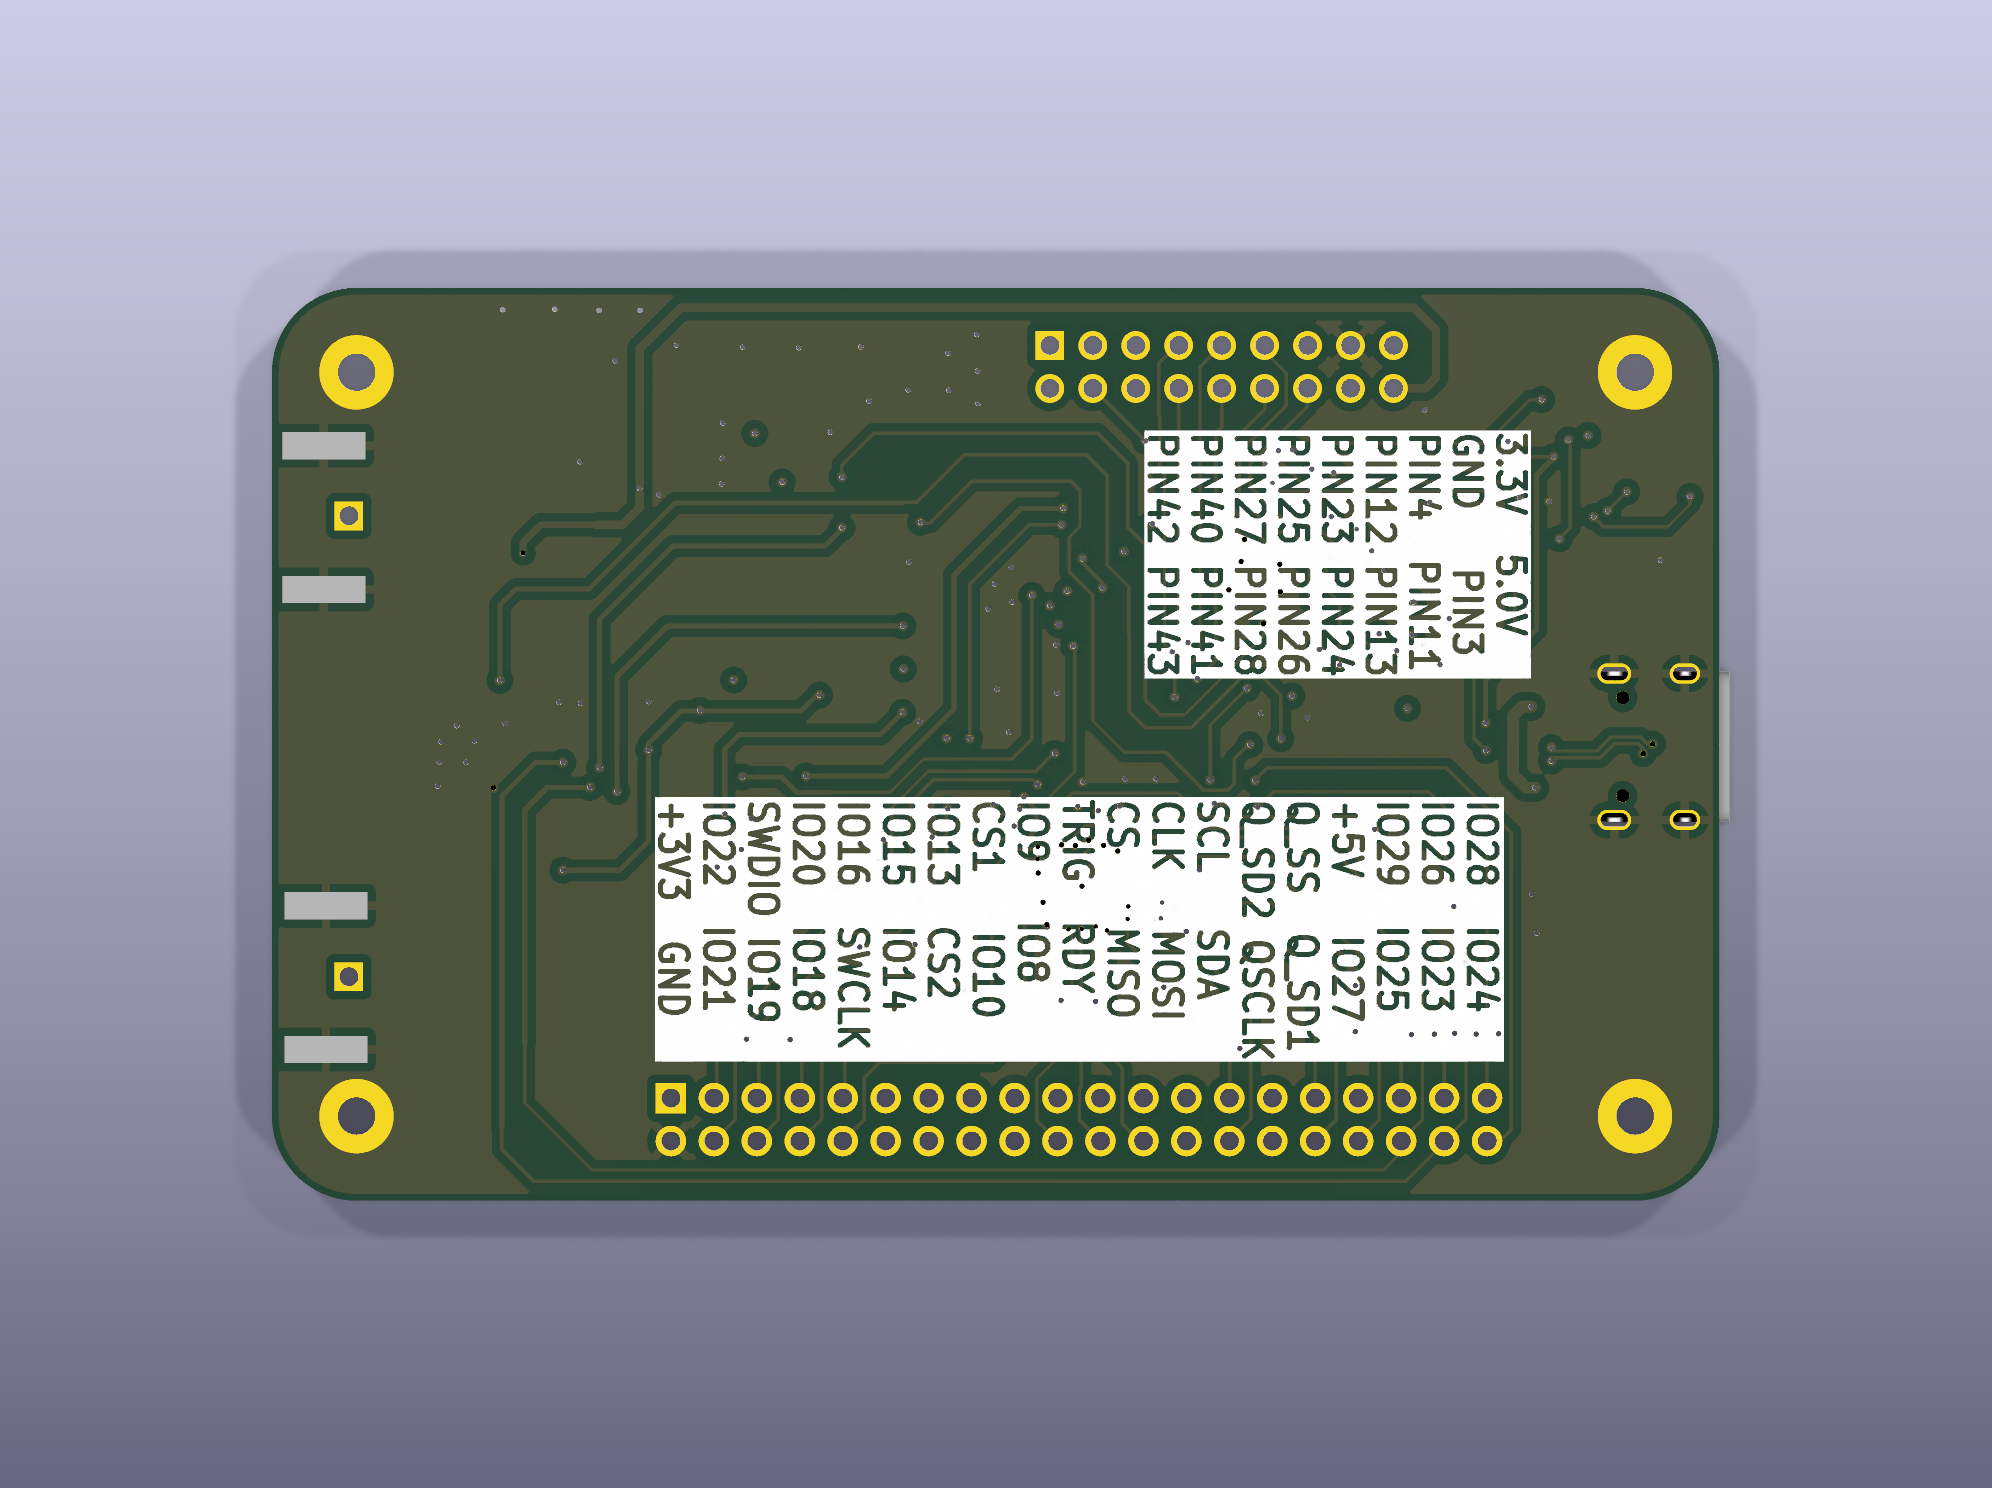
\includegraphics[width=0.48\textwidth]{figures/minUS_B.png}
\caption{Top and bottom (renders from the KiCad design; 2×N headers and SMA bodies omitted).}
\end{figure}
\small
\begin{longtable}{@{}lp{30mm}p{100mm}@{}}\toprule
\textbf{Ref} & \textbf{Type} & \textbf{Function}\\\midrule\endhead
USBC1 & USB-C receptacle & 5\,V power and USB 2.0 FS (CDC console). Sink only (CC 5.1\,kΩ).\\
RF3 / RF1 / H5 & SMA / U.FL / pin & \textbf{TX}: pulser output, net \cmd{Transducer} (Q1/Q2 drains).\\
RF22 / RF23 / H10 & SMA / U.FL / pin & \textbf{RX}: receive input, net \cmd{TRANSDUCER} (C45 series). Join TX and RX with a tee/cable for a single-element probe.\\
J1 & 1×3 socket & 1 OA1IN+ (LNA out, biased AVDD/2), 2 OA1IN−, 3 OA1OUT — probe points.\\
J2 & 1×3 socket & 1 OA2IN+, 2 OA2OUT, 3 OA2IN−.\\
H6 & 2×9 header & 1 PIC RD6/ASDA1 · 2 SCL · 3 PIC RD3/TDI · 4 PIC RD5/ASCL1 · 5 PIC OSCO · 6 PIC OSCI · 7 UART\_TX · 8 UART\_RX · 9 AD1AN8 · 10 AD2AN8 · 11 OA3IN− · 12 OA3IN+ · 13 \textbf{ADC node (PIC32\_ADC)} · 14 OA3OUT · 15 GND · 16 PIC PGC2/DACOUT1 · 17 +3.3\,V · 18 +5\,V.\\
CN1 & 2×20 IDC & RP2354A breakout: 1 +3.3\,V, 2 GND, 3/4 GPIO22/21 (PIC PGD1/PGC1), 5 SWDIO, 10 SWCLK, 6–8 GPIO19/20/18, 9 UART\_TX, 11/12 GPIO15/14, 13 GPIO13 PWM, 14/15 SPI\_CS2/CS1, 16 GPIO10, 17/18 pulser GPIO9/8, 19 TRIG, 20 RDY, 21–24 SPI CS/MISO/CLK/MOSI, 25/26 SCL/SDA, 27–32 QSPI, 33 +5\,V, 34/35/37/39 GPIO27/29/26/28, 36/38 gain mux S0/S1 (GPIO25/23), 40 GPIO24 (PIC MCLR).\\
SW1 & push button & RP2354A RUN (reset).\\
SW2 & push button & RP2354A BOOTSEL (QSPI\_SS): hold while plugging in for the UF2 drive.\\
SW3 & push button & PIC RD4 (10\,kΩ pull-up), user input — not used by the firmware.\\
LED1 & red LED & PIC RC5 via 330\,Ω: heartbeat (blinks while the PIC firmware runs).\\
U4 + U5 & RGB LED + LP5562 & I²C LED driver at 0x30 (ADDR\_SEL = GND, EN tied high); driven by \cmd{rgb R G B [pct]} since rp~1.1.1, brightness in \% since 1.1.2 (internal clock, so OSC1 is not needed).\\
H1–H4 & M2 holes & mounting, padded.\\\bottomrule
\end{longtable}
\normalsize

% ====================================================================== 6 firmware
\section{Firmware and host interface}
\subsection{Architecture}
\begin{itemize}
  \item \textbf{RP2354A} (\texttt{firmware/rp2354}, pico-sdk 2.1.0, \cmd{minus-rp2354} \rpfwrel): USB CDC console, command parser,
        pulser PIO, gain mux, RP↔PIC link, and an ICSP programmer that flashes the PIC image embedded in the RP firmware.
  \item \textbf{PIC32AK} (\texttt{firmware/pic32}, XC-DSC 3.31, \cmd{minus-pic32} \picfwrel): clocks, op amps, ADC1/ADC2, SCCP
        trigger, DMA capture, pattern correction, link protocol \vproto.
  \item Update: \cmd{reboot dfu} (or SW2 at plug-in) → copy \texttt{minus\_rp.uf2} to the RP2350 drive → \cmd{pic flash}.
        Prebuilt images are in the repository: \texttt{firmware/rp2354/build/minus\_rp.uf2}, \texttt{firmware/pic32/build/minus\_pic.hex}.
\end{itemize}

\subsection{Command reference (USB console, one line per command)}
\small
\begin{longtable}{@{}p{46mm}p{118mm}@{}}\toprule
\textbf{Command} & \textbf{Description}\\\midrule\endhead
\cmd{pe [hi [lo [in [dead]]]]} & Pulse-echo: arm the pulser on the next RDY rise, capture 4095 samples on input \cmd{in} (default 25), print header + samples; auto re-shot (≤ 8) if the sample clock locked slow. Defaults 200\,ns / 500\,ns / 25 / 27\,ns.\\
\cmd{pulse [hi [lo [dead]]]} & One pulser shot now, no capture (scope check).\\
\cmd{gain [leg [u1 [u2]]]} & Set R\textsubscript{f} leg 0–3 on both stages and unity bypass per stage; no argument: show.\\
\cmd{acq [div [samc [in [navg]]]]} & Capture without pulsing. \cmd{div}: trigger period in 5\,ns (4 = 25\,Msps, 10 = 20, 20 = 10); \cmd{samc} 0–7 sampling time; \cmd{in} input code (19 = DAC); \cmd{navg} 1–16 summed conversions (back to 1 when not given).\\
\cmd{pc [0|1]} & Fixed-pattern correction off/on; show last offsets (\S\ref{sec:pc}).\\
\cmd{env <dec> [shots [in]]} & Pulse + envelope computed on the PIC (dec 4–64), averaged over shots; 4095/dec values (\S\ref{sec:env}).\\
\cmd{envbp <dec> [shots [in [fc [bw]]]]} & Pulse + band-pass envelope on the PIC (Gaussian complex filter, default 3300 / 2500\,kHz).\\
\cmd{tof <thr> [blank\_ns [in [ref]]]} & Pulse + first threshold crossing after the blank, computed on the PIC; one line (\S\ref{sec:tof}).\\
\cmd{acqos <4|16> [in [pe]]} & Capture with ADC oversampling, 13/14-bit, 186/565\,ns per sample; not for RF echoes.\\
\cmd{tgc [off|<t\_us> <leg> …]} & Time-gain steps: gain leg switched at up to 4 times after the pulse.\\
\cmd{link [uart|spi [MHz]]}, \cmd{linktest [n [MHz]]} & Payload path and counters; SPI link self-test (\S\ref{sec:link}).\\
\cmd{fmt [text|b64]} & Sample output: decimal lines or base64 (the Python library uses b64).\\
\cmd{dac …} & PIC DAC test signal on DACOUT1 = input 19.\\
\cmd{raw LOCK?}, \cmd{raw RELOCK} & PIC PLL lock check result / redo it (\S\ref{sec:lock}).\\
\cmd{version}, \cmd{help} & Firmware, chip and unique ID; command list.\\
\cmd{ping}, \cmd{auto}, \cmd{stop}, \cmd{stat} & Link test (\cmd{PING n}→\cmd{PONG n}), periodic ping, counters.\\
\cmd{raw <text>} & Send a link line to the PIC and print the reply (e.g. \cmd{raw ID?}).\\
\cmd{pic id|flash|verify|} \cmd{erase|pins} & ICSP programmer for the PIC (pair 1, GPIO21/22/24).\\
\cmd{reset}, \cmd{reboot [dfu]} & PIC MCLR pulse; RP reboot / BOOTSEL.\\
\cmd{rgb R G B [pct]} & RGB LED colour, 0–255 per channel, LP5562 U5 on I²C at \cmd{pct}\,\% brightness (0–100, default 25 = dim, scales the PWM); reply ends \cmd{(LP5562 0x30: ok)}.\\
\cmd{i2c} & I²C bus scan (found: \vitwoc).\\
\cmd{acqcpu}, \cmd{acqil}, \cmd{raw ADCBB} & Diagnostics / experiments (CPU-loop capture, two-channel interleave, ADC throughput).\\\bottomrule
\end{longtable}
\normalsize
Input codes: 0–15 = ADC1 PINSEL, 16–31 = ADC2 PINSEL + 16. Board~3: \textbf{25} AD2AN9 ADC node (default), 17 AD2AN1 OA2OUT,
0 AD1AN0 OA1OUT, 1 AD1AN1 LNA output (aliased wideband noise, see errata), 15/31 internal band gap, 14/30 internal 15/16 AVDD.

\subsection{Data format}
\begin{lstlisting}
> pe
# acq n=4095 fill=164.7us fs=24.86Msps rp_fill=163us ... pulse-echo: pulse on RDY rise (+5V 200 / off 27 / GND 500 ns),
#   in=25 AD2AN9 (...), 40 ns/sample; gain leg 0 (Rf 2.2k) OA1 x1.00 (UGE) OA2 x3.20 = x3.2 (10.1 dB, + LNA); try 1
2019
2023
...           (4095 lines, unsigned 12-bit codes, mid-scale ~2020)
# pulse fired, 1 shot(s)
\end{lstlisting}
Host software: the Python package in \texttt{python/library} wraps every command (one method each, replies parsed into objects),
and the notebooks in \texttt{python/notebooks} walk through them step by step with the bytes on the wire. A check
(\texttt{python -m minus.fwsync}) keeps the library in step with the firmware sources.
\begin{lstlisting}
from minus import Minus            # pip install -e python/library
dev = Minus()                      # finds /dev/ttyACM*, checks both firmware versions
dev.gain(2, 0, 0)
a = dev.pe()                       # a.samples (uint16), a.t_us, a.depth_mm(), a.fs_msps, a.shots
\end{lstlisting}
One-off commands from a shell: \texttt{python3 firmware/rp2354/tools/rpcli.py /dev/ttyACM0 "gain 2 0 0" "pe" --wait=2 > shot.txt}.
With \cmd{fmt b64} the samples follow the header as \cmd{\# b64 8190} and lines of 76 base64 characters (57 bytes of u16
little-endian each). Live view: \texttt{python3 -m minus.live} (A-line, envelope, M-mode; needs a matplotlib GUI backend) or
\texttt{minus.live.LiveView(dev)} in Jupyter.

% ====================================================================== 7 application
\section{Application information}
\subsection{Getting a first A-line}
\begin{enumerate}
  \item Connect a 1–7\,MHz single-element transducer to TX and RX (tee or the U.FL pair); plug USB-C.
  \item Check: \cmd{version}, \cmd{raw ID?} (PIC answers), \cmd{ping}.
  \item \cmd{gain 0 1 0} (≈\,11\,dB) and \cmd{pe}; raise the gain until the echoes of interest use most of the ±2048 range without clipping.
  \item Average several shots on the host for weak echoes, after aligning them on a strong echo (noise falls as $1/\sqrt{N}$: \vavggain\,dB for 8 shots\meas).
\end{enumerate}
\subsection{Choosing the pulse}
A unipolar pulse of length $t$ has a spectrum $\propto |\sin(\pi f t)|$: strongest at $f_c$ for $t = 1/(2f_c)$ and nulled at
$t = 1/f_c$. The measured curve (\vhinpts{} points below 150\,ns) has its maximum at $t_{hi}$ = \vhibest\,ns and its minimum near
250\,ns — both about \vdeltaeff\,ns earlier than the ideal 155\,ns / 310\,ns at 3.22\,MHz. The effective +5\,V pulse is therefore
$t_{hi}$ + $\approx$\,\vdeltaeff\,ns: during the 27\,ns dead time nothing pulls the output down (it stays at +5\,V on the cable
capacitance) and the driver turn-on/turn-off delays add the rest. Below $\approx$\,25\,ns the driver no longer reaches full
swing (13\,ns gives almost no echo). For this probe \cmd{pe 100} gives 1.9 times the echo amplitude of the 200\,ns default;
the plateau is 75–130\,ns. The GND clamp length (0–2\,µs) changes neither the echo amplitude nor the \vdeadzone\us{} ring-down much:
the ring-down is the transducer's own; the clamp mainly defines the end state before the output is released.
\subsection{Limitations}
\begin{itemize}
  \item Throughput: one \cmd{pe} takes \xFmtBsix\,ms end to end from Python (SPI link + base64; rev 0.2: \vpetime\,s over the UART),
        \cmd{tof} \xTofTime\,ms, \cmd{env 8} \xEnvTimeA\,ms; the USB CDC buffer of the RP SDK (256 bytes) is the remaining limit.
  \item Time-gain compensation is by steps (\cmd{tgc}), each costing $\approx$\,17\us{} of switch transient.
  \item 5\,V excitation only: echoes from deep or attenuating targets need averaging.
\end{itemize}

% ====================================================================== 8 errata
\section{Known issues (errata)}
\small
\begin{tabularx}{\linewidth}{@{}lX@{}}\toprule
\textbf{ID} & \textbf{Issue and workaround}\\\midrule
E1 & \textbf{TX at +5\,V during power-up.} GPIO9 has no pull-up; the RP2350 pad default pull-down turns Q1 on until the firmware idles the pins (a few ms). Fix: 10\,kΩ pull-up on GPIO9, 10\,kΩ pull-down on GPIO8. The net names PWM\_H/PWM\_L are swapped vs function.\\
E2 & \textbf{ADC slow lock.} The 32\,ns conversion on 20\,ns triggers sometimes locks to 40/60/60\,ns. It is a per-PLL-lock state (\S\ref{sec:lock}); since pic 1.1.2 the PIC re-locks at boot until uniform and the RP sends \cmd{RELOCK} after 3 slow captures; \cmd{pe}/\cmd{acq} still re-shoot (≤ 8).\\
E3 & \textbf{Sample-comb phase} varies over one sample period from shot to shot (\vEphispan\,ns p-p, \vEphirms\,ns rms, independent shots), and the comb slips by a whole sample during \vEslipa–\vEslipb\,\% of captures (more often later in the capture; \S\ref{sec:combphase}). Align on the echo of interest before averaging. Root cause (SCCP/ADC clock-domain start) not yet fixed.\\
E4 & \textbf{Period-4 fixed pattern} on external ADC inputs (\xPcRaw\,LSB rms). Removed in firmware (\cmd{pc}, \S\ref{sec:pc}; \xPcCor\,LSB residual); a comb slip inside a capture leaves part of it in that capture. Source of the coupling not yet found.\\
E5 & \textbf{Interference lines} at 2.72\,MHz (in band) and 0.49\,MHz entering at the front end; up to half the in-band noise at high gain. Source unknown.\\
E6 & \textbf{LNA output tap (input 1)} reads 26\,mV rms of flat, aliased noise that does not reach OA1OUT: GHz-wide LNA noise or an oscillation folded by the ADC sample-and-hold. Not a valid measurement point; to check with a fast scope.\\
E7 & \textbf{RGB LED} — \emph{fixed in rp 1.1.1}: \cmd{rgb} now drives the LP5562 over I²C (the WS2812 driver on GPIO10 was for the devkit).\\
E8 & \textbf{\cmd{reboot dfu}} occasionally does not come back as the UF2 drive (seen again 2026-11-22: no USB device at all until replugged); use SW2 at plug-in.\\
E9 & U3 is fitted as MIC4427YMM (TC4427 out of stock); fixed in the design files (2026-11-21).\\
E10 & Internal 15/16\,AVDD channel reads 3480 instead of 3840 codes; internal references need SAMC ≥ 3.\\
E11 & \textbf{TX and RX are separate nets}: a single-element probe needs an external tee (R69, a 0\,Ω TX–RX link, is in the next revision).\\
E12 & \textbf{tgc switch transient}: $\approx$\,2\us{} saturation + 15\us{} settling per 4052 switch (break-before-make); a make-before-break or parallel-R\textsubscript{f} switch would remove it.\\\bottomrule
\end{tabularx}
\normalsize

% ====================================================================== 9 mechanical
\section{Mechanical}
\begin{minipage}[c]{0.5\textwidth}
\small
\begin{tabular}{@{}lp{62mm}@{}}\toprule
Outline & 85.65 × 54.03\,mm\\
Thickness & 1.6\,mm, 4 copper layers\\
Mounting & 4 × M2 (2.2\,mm, padded)\\
Components & 120 footprints, 39 R, 47 C\\
Main ICs & RP2354A (QFN-60), PIC32AK1216GC41048 (TQFP-48), BGA2817 (SC-70-6), 74HC4052 (TSSOP-16), TC4427/MIC4427 (MSOP-8), AP2112K (SOT-23-5), LP5562 (DSBGA-12)\\
Design files & \texttt{hardware/} (KiCad), JLC outputs in \texttt{hardware/production/}\\
Certification & OSHWA open source hardware, UID \textbf{FR000032}; mark + UID on the front silkscreen\\\bottomrule
\end{tabular}
\end{minipage}\hfill
\begin{minipage}[c]{0.46\textwidth}
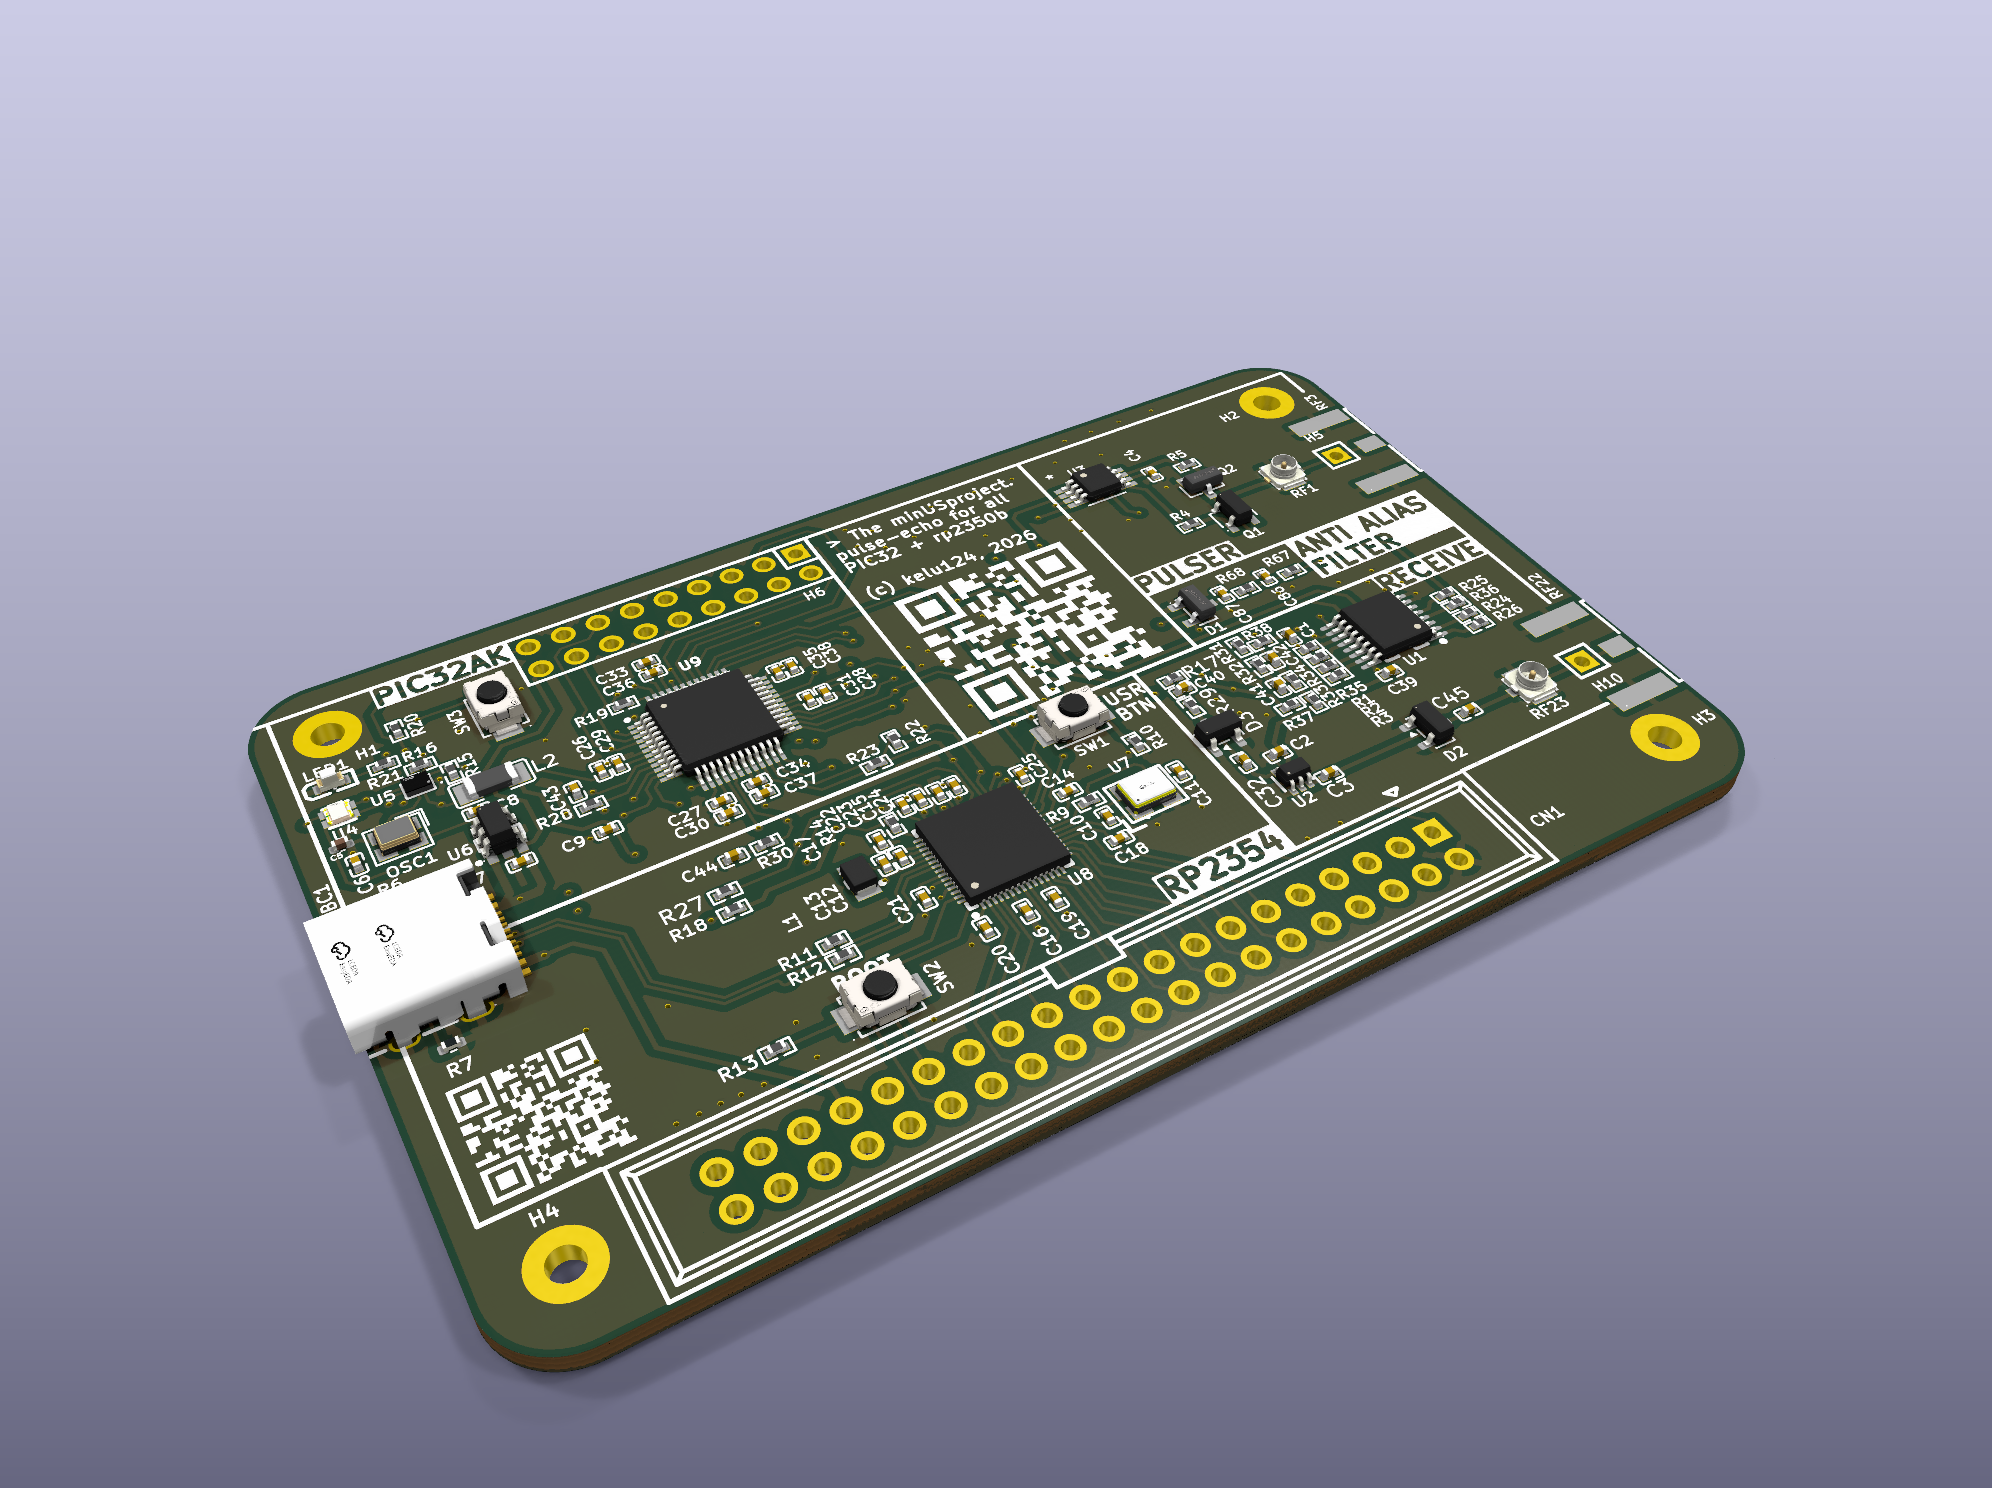
\includegraphics[width=\linewidth]{figures/minUS_angled.png}
\end{minipage}

% ====================================================================== licence
\section{License and resources}
\begin{itemize}
  \item Source, design files, firmware, bench data and this datasheet: \repo.
  \item Hardware (\texttt{hardware/}): TAPR Open Hardware License v1.0. Firmware and scripts (\texttt{firmware/}, \texttt{python/},
        bench scripts): GNU GPL v3.0 or later. Documentation, this datasheet and the bench data: CC BY-SA 4.0.
        Full texts in \texttt{LICENSES/}; third-party parts (EasyEDA 3D models, Pico SDK, Microchip DFP) keep their own licenses
        (\texttt{LICENSE.md}).
  \item \textbf{OSHWA certified} open source hardware, UID \textbf{FR000032} (2026-11-20),
        \url{https://certification.oshwa.org/fr000032.html}. The certification mark is used under the OSHWA mark license agreement.
  \item \textbf{Not a medical device.} For research, education and non-destructive testing only.
\end{itemize}
\begin{center}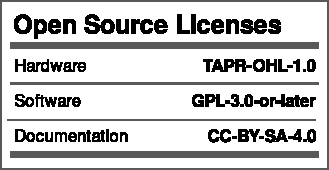
\includegraphics[height=3.6cm]{figures/oshw_facts.pdf}\hspace{1cm}
\includegraphics[height=3.6cm]{figures/FR000032.pdf}\end{center}

% ====================================================================== 10 revision
\section{Revision history}
\small
\begin{tabular}{@{}lll@{}}\toprule
\textbf{Rev} & \textbf{Date} & \textbf{Change}\\\midrule
0.1 & 2026-11-19 & First release: board 3 bring-up, firmware rp \vrpfw{} / pic \vpicfw, measurements of session 11.\\
0.2 & 2026-11-19 & Board named v1.1; firmware rp 1.1.2 / pic 1.1.0 (LP5562 \cmd{rgb} with brightness, E7 fixed); Python library + notebooks;\\
    &            & E3 sample-comb phase study (400 shots); licenses and repository links; Annex A test transducer.\\
0.3 & 2026-11-22 & Firmware rp \rpfwrel{} / pic \picfwrel{} (proto 14): SPI capture link + base64 host output; on-PIC envelope, time of\\
    &            & flight and oversampling; time-gain steps; DAC test signal; PLL lock check (E2); period-4 correction explained;\\
    &            & new measurements with the transducer (\texttt{docs/bench/2026-11-22-datasheet-ext/}).\\\bottomrule
\end{tabular}

\newpage
% ====================================================================== annex A
\section*{Annex A — Test transducer}\label{sec:piezo}
\addcontentsline{toc}{section}{Annex A — Test transducer}
Every \meas{} value in this datasheet was taken with the same single-element piezo probe (``BiVi piezo'', 3.3\,MHz nominal),
on TX and RX. Its one-port reflection was measured by the owner with a NanoVNA
(\texttt{datasheet/piezo\_test/BiViPiezo.s1p}: \vPnpts{} points, \vPfmin–\vPfmax\,MHz, S\textsubscript{11} re/im, 50\,Ω). The values
below come from \texttt{datasheet/piezo\_test/analyze\_s1p.py}. The measurement is at the VNA port, so it includes any cable or adapter.

\small
\begin{longtable}{@{}p{62mm}p{60mm}r@{}}\toprule
\textbf{Parameter} & \textbf{How} & \textbf{Value}\\\midrule\endhead
Return-loss dip 1 & minimum of |S\textsubscript{11}| & \vPdipa\,MHz, \vPrla\,dB, Z = \vPza\,Ω\\
Return-loss dip 2 & second minimum & \vPdipb\,MHz, \vPrlb\,dB, Z = \vPzb\,Ω\\
Return loss between the dips & worst point between them & \vPmidrl\,dB at \vPmidf\,MHz\\
Return loss ≥ 10\,dB & (VSWR ≤ 1.92) & \vPsubs\,MHz\\
|Z| over 3.0–4.4\,MHz & & \vPzlo–\vPzhi\,Ω\\
Impedance at 3.30\,MHz & & \vPzmag\,Ω, \vPzph°\\
Conductance peak & max Re(1/Z) & \vPfs\,MHz\\
Resistance peak & max Re(Z) & \vPfp\,MHz\\
Phase zero crossings & & \vPzc\,MHz\\\bottomrule
\end{longtable}
\normalsize
The probe looks \textbf{electrically matched to 50\,Ω}: |Z| stays within \vPzlo–\vPzhi\,Ω across 3–4.4\,MHz, the response loops round
the centre of the Smith chart, and away from resonance the susceptance is inductive. A bare ceramic would be capacitive there, so a
Butterworth–Van Dyke fit of the element itself does not apply. The double dip is typical of a matched, damped probe. The acoustic
echo band measured through the board (electrical characteristics, ``Echo −6\,dB band'': \vbwlo–\vbwhi\,MHz, peak
\vfpeak\,MHz) sits on the lower dip. The 200\,ns unipolar pulse, the two-way transducer response and the RX anti-alias filter all
weight the echo spectrum towards lower frequencies.
\begin{figure}[h]\centering
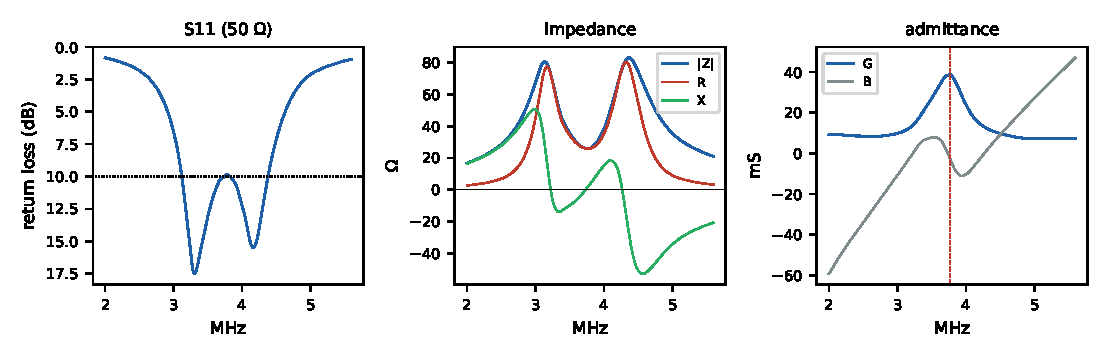
\includegraphics[width=\textwidth]{figures/piezo_impedance.pdf}\\[2pt]
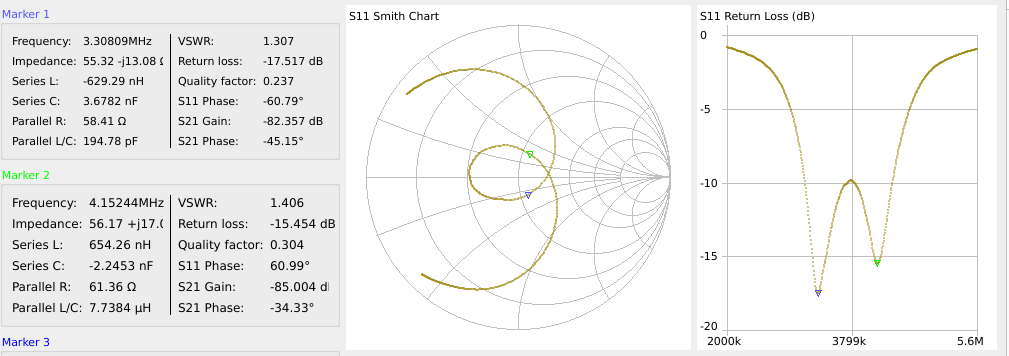
\includegraphics[width=0.9\textwidth]{figures/piezo_vna.png}
\caption{Test transducer, S\textsubscript{11} from \texttt{BiViPiezo.s1p}. Top: return loss, impedance (|Z|, R, X), admittance (G, B;
dashed = conductance peak). Bottom: the NanoVNA screen as measured (markers at the two return-loss dips).}
\end{figure}

\end{document}
